% /*
%  * ----------------------------------------------------------------------------
%  * "THE BEER-WARE LICENSE" (Revision 42):
%  * <michi.wieland@hotmail.com> wrote this file. As long as you retain this notice you
%  * can do whatever you want with this stuff. If we meet some day, and you think
%  * this stuff is worth it, you can buy me a beer in return. Michael Wieland
%  * ----------------------------------------------------------------------------
%  */

\documentclass[
a4paper,
oneside,
10pt,
fleqn,
headsepline,
toc=listofnumbered, 
bibliography=totocnumbered]{scrartcl}

% deutsche Trennmuster etc.
\usepackage[T1]{fontenc}
\usepackage[utf8]{inputenc}
\usepackage[english, ngerman]{babel} % \selectlanguage{english} if  needed
\usepackage{lmodern} % use modern latin fonts

% Custom commands
\newcommand{\AUTHOR}{Michael Wieland}
\newcommand{\INSTITUTE}{Hochschule für Technik Rapperswil}
\newcommand{\GITHUB}{https://github.com/michiwieland/hsr-zusammenfassungen}
\newcommand{\LICENSEURL}{https://en.wikipedia.org/wiki/Beerware}
\newcommand{\LICENSE}{
"THE BEER-WARE LICENSE" (Revision 42):
<michi.wieland@hotmail.com> wrote this file. As long as you retain this notice you
can do whatever you want with this stuff. If we meet some day, and you think
this stuff is worth it, you can buy me a beer in return. Michael Wieland	
}

% Jede Überschrift 1 auf neuer Seite
\let\stdsection\section
\renewcommand\section{\clearpage\stdsection}

% Multiple Authors
\usepackage{authblk}

% Include external pdf
\usepackage{pdfpages}

% Layout / Seitenränder
\usepackage{geometry}

% Inhaltsverzeichnis
\usepackage{makeidx} 
\makeindex

\usepackage{url}
\usepackage[pdfborder={0 0 0}]{hyperref}
\usepackage[all]{hypcap}
\usepackage{hyperxmp} % for license metadata

% Glossar und Abkürzungsverzeichnis
\usepackage[acronym,toc,nopostdot]{glossaries}
\glossarystyle{altlist}
\usepackage{xparse}
\DeclareDocumentCommand{\newdualentry}{ O{} O{} m m m m } {
	\newglossaryentry{gls-#3}{
		name={#4 : #5},
		text={#5\glsadd{#3}},
		description={#6},
		#1
	}
	\makeglossaries
	\newacronym[see={[Siehe:]{gls-#3}},#2]{#3}{#4}{#5\glsadd{gls-#3}}
}
\makeglossaries

% Mathematik
\usepackage{amsmath}
\usepackage{amssymb}
\usepackage{amsfonts}
\usepackage{enumitem}

% Images
\usepackage{graphicx}
\graphicspath{{images/}} % default paths

% Boxes
\usepackage{fancybox}

%Tables
\usepackage{tabu}
\usepackage{booktabs} % toprule, midrule, bottomrule
\usepackage{array} % for matrix tables

% Multi Columns
\usepackage{multicol}

% Header and footer
\usepackage{scrlayer-scrpage}
\setkomafont{pagehead}{\normalfont}
\setkomafont{pagefoot}{\normalfont}
\automark*{section}
\clearpairofpagestyles
\ihead{\headmark}
\ohead{\AUTHOR}
\cfoot{\pagemark}

% Pseudocode
\usepackage{algorithmic}
\usepackage[linesnumbered,ruled]{algorithm2e}

% Code Listings
\usepackage{listings}
\usepackage{color}
\usepackage{beramono}

\definecolor{bluekeywords}{rgb}{0,0,1}
\definecolor{greencomments}{rgb}{0,0.5,0}
\definecolor{redstrings}{rgb}{0.64,0.08,0.08}
\definecolor{xmlcomments}{rgb}{0.5,0.5,0.5}
\definecolor{types}{rgb}{0.17,0.57,0.68}

\lstdefinestyle{visual-studio-style}{
	language=[Sharp]C,
	columns=flexible,
	showstringspaces=false,
	basicstyle=\footnotesize\ttfamily, 
	commentstyle=\color{greencomments},
	morekeywords={partial, var, value, get, set},
	keywordstyle=\bfseries\color{bluekeywords},
	stringstyle=\color{redstrings},
	breaklines=true,
	breakatwhitespace=true,
	tabsize=4,
	numbers=left,
	numberstyle=\tiny\color{black},
	frame=lines,
	showspaces=false,
	showtabs=false,
	escapeinside={£}{£},
}

\definecolor{DarkPurple}{rgb}{0.4, 0.1, 0.4}
\definecolor{DarkCyan}{rgb}{0.0, 0.5, 0.4}
\definecolor{LightLime}{rgb}{0.3, 0.5, 0.4}
\definecolor{Blue}{rgb}{0.0, 0.0, 1.0}

\lstdefinestyle{cevelop-style}{
	language=C++,  
	columns=flexible,
	showstringspaces=false,     
	basicstyle=\footnotesize\ttfamily, 
	keywordstyle=\bfseries\color{DarkPurple},
	commentstyle=\color{LightLime},
	stringstyle=\color{Blue}, 
	escapeinside={£}{£}, % latex scope within code      
	breaklines=true,
	breakatwhitespace=true,
	showspaces=false,
	showtabs=false,
	tabsize=4,
	morekeywords={include,ifndef,define},
	numbers=left,
	numberstyle=\tiny\color{black},
	frame=lines,
}

\lstdefinestyle{eclipse-style}{
	language=Java,  
	columns=flexible,
	showstringspaces=false,     
	basicstyle=\footnotesize\ttfamily, 
	keywordstyle=\bfseries\color{DarkPurple},
	commentstyle=\color{LightLime},
	stringstyle=\color{Blue}, 
	escapeinside={£}{£}, % latex scope within code      
	breaklines=true,
	breakatwhitespace=true,
	showspaces=false,
	showtabs=false,
	tabsize=4,
	morekeywords={length},
	numbers=left,
	numberstyle=\tiny\color{black},
	frame=lines,
}
\lstset{style=eclipse-style}



% Theorems \begin{mytheo}{title}{label}
\usepackage{tcolorbox}
\tcbuselibrary{theorems}
\newtcbtheorem[number within=section]{definiton}{Definition}%
{fonttitle=\bfseries}{def}
\newtcbtheorem[number within=section]{remember}{Merke}%
{fonttitle=\bfseries}{rem}
\newtcbtheorem[number within=section]{hint}{Hinweis}%
{fonttitle=\bfseries}{hnt}

% Dokumentinformationen
\newcommand{\SUBJECT}{Zusammenfassung}
\newcommand{\TITLE}{Informationssicherheit 2}

\loadglsentries{glossar}

% pdf metadata
\hypersetup{
	pdfauthor={\AUTHOR},
	pdftitle={\SUBJECT \TITLE},
	pdfcopyright={\LICENSE},
	pdflicenseurl={\LICENSEURL}
}

\begin{document}
	
% Front page
\title{\TITLE}
\subject{\SUBJECT}
\author{\AUTHOR}
\affil{\INSTITUTE}
\date{\today}
\maketitle

\vfill

% Participate
\paragraph{Mitmachen} \hfill \\
Falls Du an diesem Dokument mitarbeiten willst, kannst Du das Dokument
auf GitHub unter \url{\GITHUB} forken.

% Licence
\paragraph{Lizenz} \hfill \\
\LICENSE

% Table of contents
\tableofcontents


% Glossar and acronyms (if included \loadglsentries{glossar})
\printglossary[type=\acronymtype]
\printglossary
\glsaddall


\section{Grundlagen}
\subsection{OSI Stack}
\begin{figure}[h]
\centering
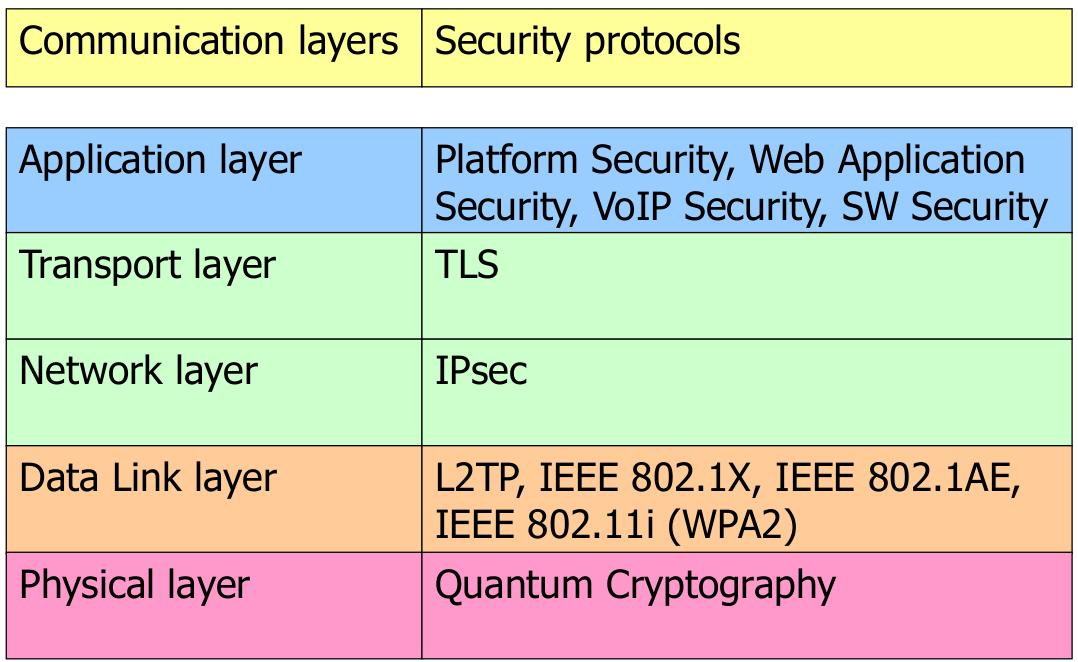
\includegraphics[width=0.5\linewidth]{images/sec_osi_stack}
\caption{OSI Stack}
%\label{fig:secosistack}
\end{figure}

\subsection{Kryptographiesche Stärken}
\paragraph{Kryptographiesche Stärken} \hfill
\begin{figure}[h!]
\centering
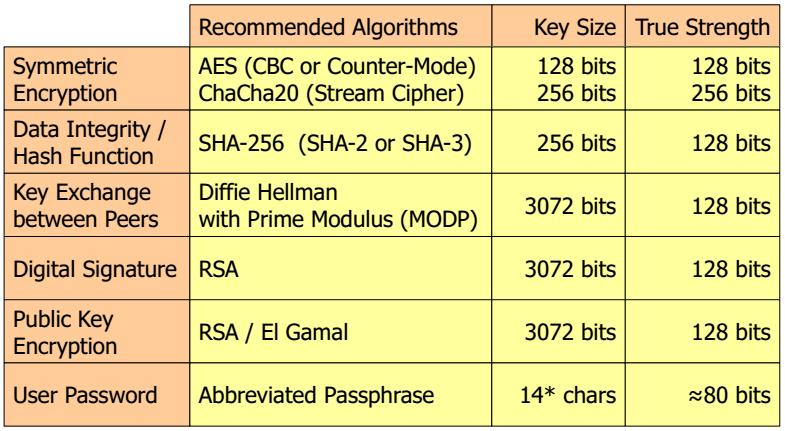
\includegraphics[width=0.5\linewidth]{images/cryptographical_strenght}
\caption{Kryptograpische Schlüssel Stärken}
\label{fig:cryptographicalstrenght}
\end{figure}

\paragraph{Schlüssellängen} \hfill
\begin{figure}[h!]
\centering
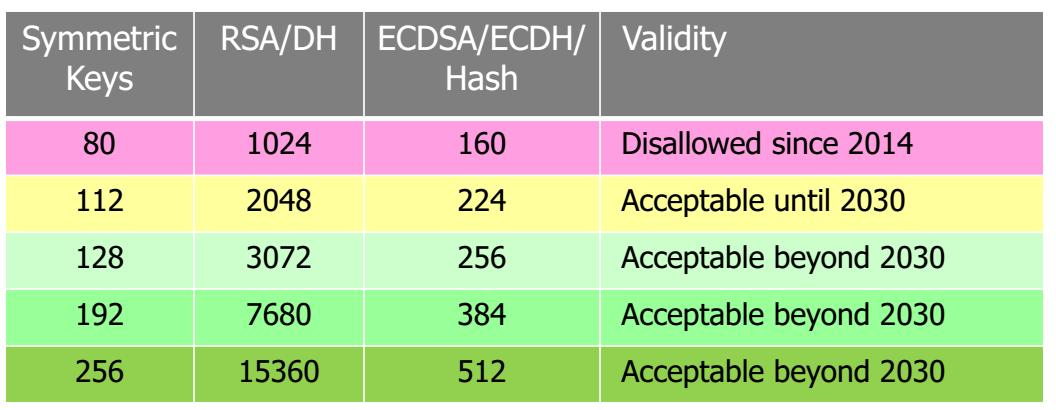
\includegraphics[width=0.5\linewidth]{images/key_strenght_comparison}
\caption{NIST 2012 Comparative Security Strength}
\label{fig:keystrenghtcomparison}
\end{figure}
\begin{hint}{NIST 2012 Compartive Security Strenght}{}
	Diese Grafik muss auswendig gelernt werden. Kommt garantiert an der Prüfung
\end{hint}

\subsection{NSA Suite B}
Die Suite B ist eine Sammlung an kryptographischer Algorithmen, die 2005 von der NSA veröffentlicht wurde. Die Suite A wurde aktuell (2016
) noch nicht veröffentlicht.

\section{Verschlüsselungsverfahren}
\subsection{Speed}
Wird für die Verschlüsselung die Hardwarebeschleunigung AES-NI verwendet ist ein Performancegewinn von ca. Faktor 2-3 zu erkennen.
\begin{table}[h]
	\centering
	\begin{tabu} to \linewidth {l l X}
		\toprule 
		Ranking & Verfahren & Bemerkung \\
		\midrule
		1 & AES-GCM & \\
		2 & AES & Je kleiner die Schlüssellänge desto schneller. Je kleiner die Schlüssellänge desto weniger Runden (10, 12, 14) \\
		3 & Camellia & Konservativer gewählte Rundenanzahl (18, 24) \\
		4 & DES & \\
		5 & 3DES & 12-13 mal langsamer als AES-128 \\
		\bottomrule 
	\end{tabu} 
	\caption{Speed von Verschlüsselungsverfahren}
\end{table}

\subsection{Symmetrisch}
\subsubsection{AES: Advanced Encryption Standard}
\begin{itemize}
	\item Block Cipher mit einer Blockgrösse von 128 Bit
	\item Es gibt drei Varianten von Schlüssellängen, welche sich nur in den Anzahl Runden unterscheiden
	\begin{enumerate}
		\item 128Bit: 10Runden
		\item 192Bit: 12Runden
		\item 256Bit: 14Runden
	\end{enumerate}
	\item Neuere Intel CPUs unterstützen das \gls{aes-ni} (Hardwarebeschleunigung) Instruktionsset, welches den Algorithmus um Faktor zwei bis drei schneller macht. Dieser Modus ist standardmässig aktiviert.
	\item AES GCM ermöglicht eine Verschlüsselung des Plaintextes und garantiert die Integrität des generierten Ciphertextes, sowie zusätzlicher unverschlüsselter Daten durch eine kryptographische Checksumme. AES GCM hat einen hohen Datendurchsatz, weshalb dieser Modus gerne bei TLS Zertifikaten an den Anfang der Liste gesetzt wird.  Einerseits können alle Counter-Blöcke vorberechnet werden, sobald der IV und die Plaintext-Länge bekannt sind. Andererseits kann die Authentisierung von Ciphertext-Blöcken und die Verschlüsselung von weiteren Plaintext-Blöcken parallel ablaufen.
\end{itemize}

\paragraph{AES CTR: Counter Mode}
Der Counter Mode ist eine Betriebsart, in der Blockchiffren wie AES betrieben werden können, um daraus eine Stromchiffren zu erzeugen. Zur Verschlüsselung wird ein Initialisierungsvektor mit dem Schlüssel verschlüsselt und so ein Zwischenschlüssel produziert. Dieser wird im Anschluss mittels einer XOR-Operation mit dem Klartext kombiniert. Daraus entsteht der Geheimtext.



\subsubsection{Camellia}
Camellia verwendet die gleichen Parameter wie AES: eine Blockgröße von 128 Bit und Schlüssellängen von 128, 192 oder 256 Bit. Camellia wurde in Japan entwickelt und kann mit AES verglichen werden. Im Zweifelsfall sollte aber AES verwendet werden, da dieses Verfahren weiter verbreitet ist, und die Hardware eher für AES optimiert ist.
\begin{itemize}
	\item Block Cipher mit einer Blockgrösse von 128 Bit
	\item Es gibt drei Varianten von Schlüssellängen, welche sich nur in den Anzahl Runden unterscheiden
	\begin{enumerate}
		\item 128Bit: 18Runden
		\item 192Bit: 24Runden
		\item 256Bit: 24Runden
	\end{enumerate}
\end{itemize}

\subsection{Asymmetrisch}
\subsubsection{RSA}
\gls{rsa} ist ein asymmetrisches kryptographisches Verfahren, das sowohl zum Verschlüsseln als auch zum digitalen Signieren verwendet werden kann.
\begin{itemize}
	\item RSA Signatur Schlüssel haben üblicherweise einen sehr kleinen öffentlichen Exponenten, bei dem nur zwei Bits auf 1 gesetzt sind. Im Gegensatz dazu ist das Modul und der private Exponent sehr gross, bei welchen etwa die Hälfte der Bits auf 1 gesetzt sind. Daraus resultiert, dass die Verifikation der Signatur sehr viel einfacher und schneller geht, wie die Generierung.
\end{itemize}

\paragraph{Vorgehen}
\begin{enumerate}
	\item Zwei Primzahlen wählen und Produkt bilden: $n = p \cdot q$
	\item $\varphi(n) = (p - 1) \cdot (q - 1)$
	\item Beliebige Zahl a wählen, wobei a teilerfremd zu $\varphi(n)$ sein muss. ($ggt(\varphi(n), a) = 1$) \\ $\Rightarrow$ am besten eignen sich Primzahlen für a. (privater Schlüssel)
	\item Multiplikative Inverse b berechnen (öffentlicher Schlüssel) $a \cdot b = 1$ mod $\varphi(n)$ $\Rightarrow$ erweiterter Euklidischer Algorithmus
	\begin{enumerate}
		\item Modul: n (öffentlich)
		\item Öffentlicher Schlüssel: b
		\item Privater Schlüssel: a
	\end{enumerate}	
\end{enumerate}

\paragraph{Verschlüsseln}
\begin{enumerate}
	\item $\text{Wert}_\text{verschlüsselt} = (\text{Wert}_\text{unverschlüsselt})^{b} \cdot mod(n)$
\end{enumerate}

\paragraph{Entschlüsseln}
\begin{enumerate}
	\item $\text{Wert}_\text{unverschlüsselt} = (\text{Wert}_\text{verschlüsselt})^{a} \cdot mod(n)$
\end{enumerate}

\newpage

\subsubsection{DH: Diffie-Hellman}
DH ist ein asymmetrisches Verfahren, welches dazu verwendet wird einen symmetrischen Key zu generieren. Die Idee 
hinter diesem Verfahren ist, dass die beiden Partner gemeinsam den geheimen Schlüssel generieren (Shared Master Secret), ohne ihn 
ganz übermitteln zu müssen.

\paragraph{Vorgehen}
\begin{enumerate}
	\item One Way Function: $f(x) = g^x \text{ mod p}$
	\item Die Zahlen g und p sind öffentlich und können ungeschützt übertragen werden
	\item Alice und Bob einigen sich auf die Zahlen p und g
	\item Alice wählt eine zufällige Zahl a und sendet Bob den berechneten Wert gross A. $ A = g^a { mod(p)}$
	\item Bob wählt eine zufällige Zahl b und sendet Alice den berechneten Wert gross B. $ B = g^{b}{ mod(p)} $
	\item Beide können nun den geheimen symmetrischen Schlüssel K berechnen: $K= A^{b}{ mod(p)} $ rsp. $K= B^{a}{ mod(p)} $
\end{enumerate}


\section{Hashverfahren}
\subsection{Speed}
Auf 64Bit Plattformen ist SHA-3 512 schneller wie die SHA-2 256 Variante, da sie intern 64 Bit Wörter verwendet und die 256 nur 32Bit Wörter
\begin{table}[h]
	\centering
	\begin{tabu} to \linewidth {c l}
		\toprule 
		Ranking & Verfahren \\
		\midrule
		1 & MD5 \\
		2 & SHA-1 \\
		3 & SHA-2 \\
		4 & SHA-3 \\
		\bottomrule 
	\end{tabu} 
	\caption{Speed von Hashverfahren}
\end{table}

\subsection{MD5}
MD5 (Message Digest \#5) berechnet einen 128Bit langen Hash Wert. Er darf heutzutage nicht mehr verwendet werden, da er offiziell als gebrochen gilt. (seit 2013)

\subsection{SHA-1 }
SHA-1 (Secure Hash Algorithm) berechnet einen 160Bits langen Hash Wert. NIST empfiehlt seit 2005 SHA-1 nicht mehr zu verwenden. 

\subsection{SHA-2}
Es existieren 4 SHA-2 Implementierungen (Secure Hash Algorithm Family) mit unterschiedlichen Hash Längen (SHA-224, SHA-256, SHA-384 und SHA-512). Die SHA-2 Variationen haben immer genau die halbe Schlüsselstärke (SHA-384 $\Rightarrow$ Schlüsselstärke = 192Bits). Obschon SHA-2 noch weit verbreitet ist, sollte man nicht mehr auf SHA-2 setzen.

\subsection{SHA-3}
Es existieren 4 SHA-3 (Keccak) Implementierungen mit unterschiedlichen Hash Längen (SHA3-224, SHA3-256, SHA3-384 und SHA3-512). SHA-3 ist der Gewinner eines NIST Wettbewerbs und wurde 2015 standardisiert. Keccak basiert nicht mehr auf dem ursprünglichen SHA.


\section{Elliptic Curves}
\begin{itemize}
	\item Die Schlüsselstärke ist immer die Hälfte der angegeben Schlüssellänge. (z.B ECDH256 $\Rightarrow$ 128bit)
	\item ECRSA ist wesentlich schneller wie RSA
	\item Mit dem D-Wave sind 1000Qbits möglich, jedoch wird der Shor's Quantum Algorithm nicht erfüllt, da nicht richtige Quantenzustände verwendet werden.
\end{itemize}

\subsection{Kryptografische Stärke}
Die kryptografische Stärke des ECDH Algorithmus beruht darauf, dass es sehr aufwändig ist, die Anzahl Additionen eines Kurvenpunktes $P$ mit sich selber Modulo einer Primzahl $p$ (d.h., das $n$ in $nP \mod p = (P_1 + P_2 + ... + P_n) \mod p$) herauszufinden.

Grundsätzlich baut ECDH damit auf das gleiche bzw. ein sehr ähnliches Problem wie DH und RSA auf, allerdings ist ECDH gegen einige Angriffe resistent, welche die Faktorisierung von RSA/DH einfacher machen. Dadurch sind deutlich kürzere Schlüssel möglich.

\subsection{Gruppe}\label{sec:gruppe}
Eine Gruppe ist ein algebraisches System bestehend aus G und einer Operation *, sodass für alle Elemente a,b,c in G folgende Bedingungen gelten:
\begin{enumerate}
	\item a * b muss in G sein
	\item a * (b * c) = (a * b) * c
	\item Es gibt ein Neutrales Element $\Rightarrow$ a * e = e * a = a (z.B 0 bei einer Addition)
	\item Es gibt ein Inverses Element $\Rightarrow$ a * a' = a' * a = e (z.B a'=-a bei einer Addition)
	\item Man spricht von einer Abelschen Gruppe wenn gilt: a * b = b * a (Kommutativgesetz)
\end{enumerate}

\begin{figure}[ht!]
	\centering
	\begin{minipage}[t]{0.4\textwidth}
		\centering
		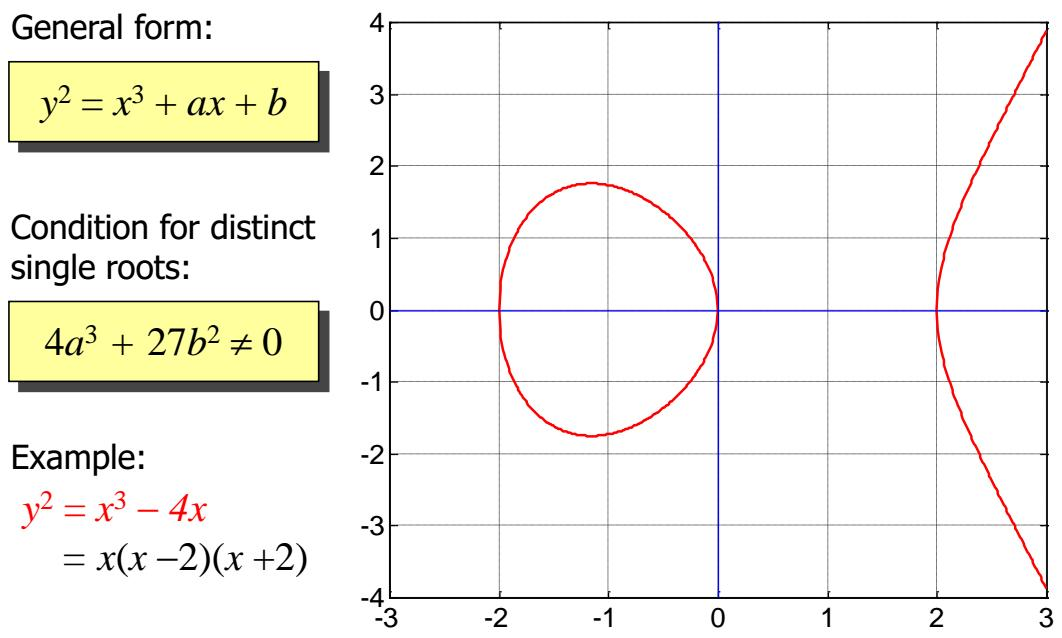
\includegraphics[width=\linewidth]{images/eliptic_curve_calculation}
		\caption{Elliptische Kurven Berechnung}
		\label{fig:elipticcurvecalculation}
	\end{minipage}
	\begin{minipage}[t]{0.4\textwidth}
		\centering
		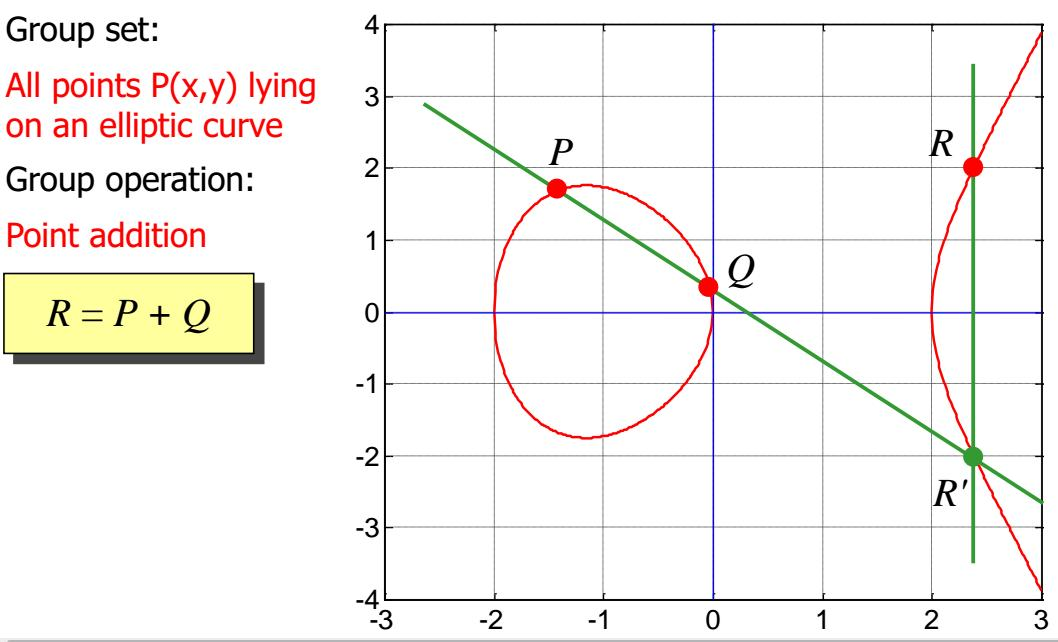
\includegraphics[width=\linewidth]{images/eliptic_curve_calculation2}
		\caption{Berechnung der Gruppe}
		\label{fig:elipticcurvecalculation2}
	\end{minipage}
\end{figure}

\begin{figure}[ht!]
	\centering
	\begin{minipage}[t]{0.4\textwidth}
		\centering
		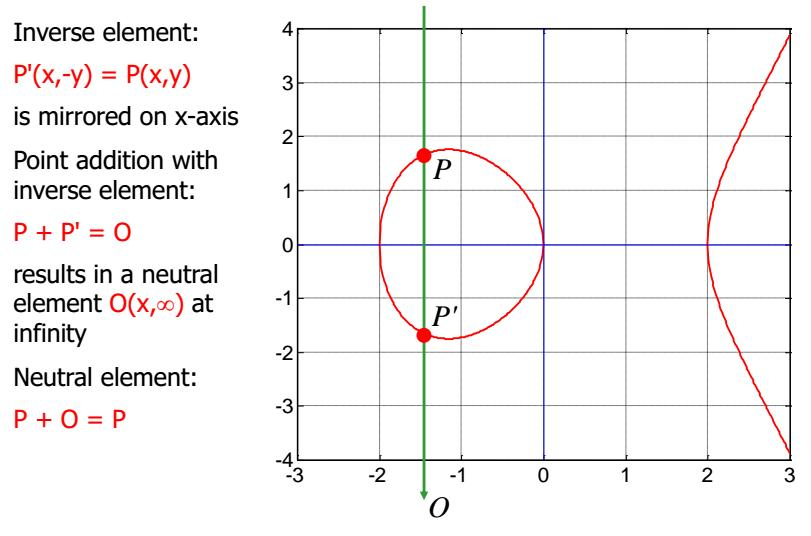
\includegraphics[width=\linewidth]{images/eliptic_curve_calculation_neutral_inverse_elem}
		\caption{Inverses und Neutrales Element}
		\label{fig:elipticcurvecalculationneutralinverseelem}
	\end{minipage}
	\begin{minipage}[t]{0.4\textwidth}
		\centering
		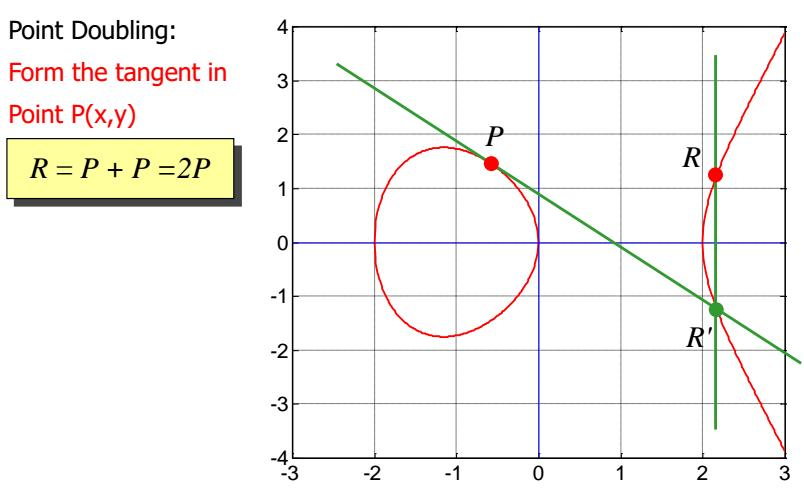
\includegraphics[width=\linewidth]{images/eliptic_curve_calculation_point_doubling}
		\caption{Q und P werden so verschoben, dass sie eine Tangente bildern}
		\label{fig:elipticcurvecalculationpointdoubling}
	\end{minipage}
\end{figure}

\begin{figure}[ht!]
	\centering
	\begin{minipage}[t]{0.4\textwidth}
		\centering
		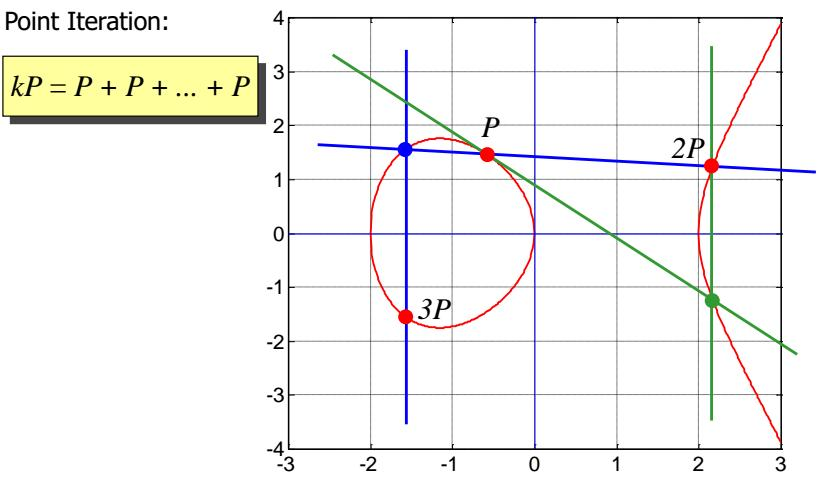
\includegraphics[width=\linewidth]{images/eliptic_curve_calculation_point_iteration}
		\caption{Point Iteration: Einen Punkt k-1 mal zu sich selbst hinzufügen}
		\label{fig:elipticcurvecalculationpointiteration}
	\end{minipage}
	\begin{minipage}[t]{0.4\textwidth}
		\centering
		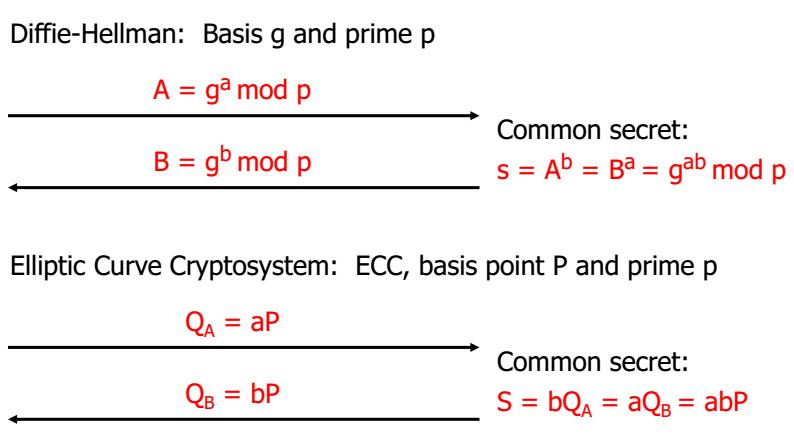
\includegraphics[width=\linewidth]{images/eliptic_curve_key_exchange}
		\caption{Schlüsselaustausch}
		\label{fig:elipticcurvekeyexchange}
	\end{minipage}
\end{figure}

\newpage
\subsection{ECDH}
Die Schwierigkeit bei ECDH ist es, die Anzahl Punktadditionen herauszufinden (privater Teil)

\begin{enumerate}
	\item Alice und Bob einigen sich auf eine Elliptische Kurve, einen Punkt auf der Kurve $P$ aus der Zahlengruppe $G$ (siehe Sektion \ref{sec:gruppe}). Diese werden ungeschützt übertragen.
	\item Alice wählt eine zufällige geheime Zahl $a$, Bob wählt eine zufällige geheime Zahl $b$
	\item Alice übermittelt Bob den ''Public Key'' $A = aP$, Bob übermittelt Alice seinen ''Public Key'' $B = bP$ über einen ''öffentlichen'' Kanal.
	\item Alice und Bob können nun mithilfe der vorhandenen Zahlen den gemeinsamen geheimen Schlüssel ausrechnen: $\text{ (Alice:) } aB = \text{ (Bob:) } bA = abP$.
\end{enumerate}

\subsection{Curve25519}
$y^2 = x^3 + 486662x^2 + x$ in einem endlichen Körper modulo der Primzahl $2^{255} - 19$

\section{Physical Layer Security}
Auf dem Physical Layer gibt es nur Quanten Kryptographie das kryptographisch sicher ist. Zusätzlich gibt es noch Frequency Hopping, welches aber nicht sicher ist, wenn man das ganze Frequenzspektrum überwachen kann. Trotzdem wird es noch in der Schweizer Armee für die Funkgeräte eingesetzt.

\subsection{Quanten Kryptographie}
Bei der Quanten Kryptographie nutzt man die Eigenschaften der Quantenmechanik, damit zwei Parteien eine gemeinsame Zufallszahl generieren können, die als geheimer Schlüssel verwendet werden kann. Quanten können nicht geklont werden. Das bedeutet, dass es erkannt werden kann, wenn die Leitung abgehört wird. Ein Qubit kann nur zwei durch Messung sicher unterscheidbare Zustände haben. (Polarisation)

\subsubsection{Ekert E91 Protokoll}
Laser erzeugt von Zeit zu Zeit ein verstränktes (entangled) Photonenpaar. Wenn man den Zustand des einen misst, kennt man den Zustand des anderen. Beide Entstationen müssen mit dem gleichen Filterset messen (vertikal, horizontal). Wenn mehrere Photonen nicht ankommen (einzelne können von der Glasfaser geschluckt werden), kann der Empfänger davon ausgehen, dass die Leitung abgehört wird. Das Protokoll funktioniert aber nur auf Distanzen bis ca. 10km.
\begin{figure}[h]
\centering
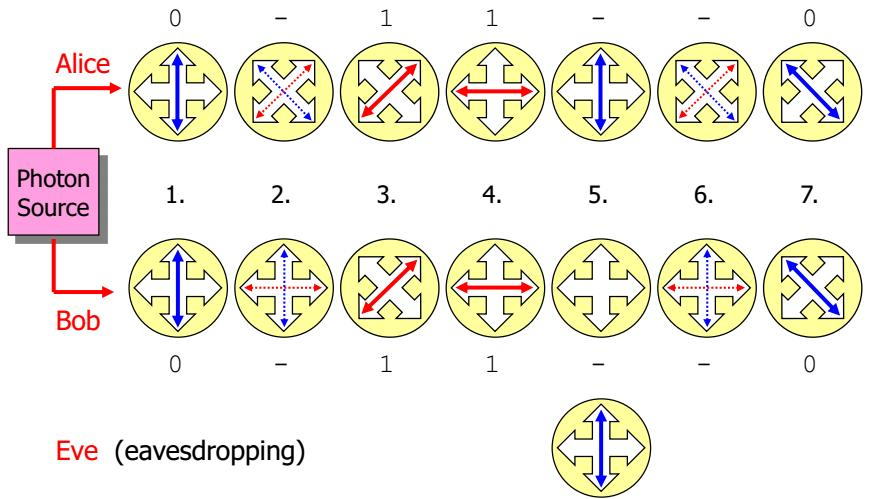
\includegraphics[width=0.5\linewidth]{images/entangled_photons}
\caption{Entangled Photons}
\label{fig:entangledphotons}
\end{figure}

\paragraph{Decoy States}
Um zu verschleiern, dass Photonen gestolen wurden, könnte ein Angreifer bewusst Decoy States einfügen. Als Gegenmassnahme fügt der Sender zufällige Decoy States ein und sagt dem Empfänger welches die Decoy States waren. Die Decoy States werden auf einem niedrigeren Leitungspegel ausgesendet. Wenn der Angreifer auf der Leitung sitzt, resultiert eine andere statistische Verteilung (von Daten und Decoy Pulsen), was wiederum erkannt werden kann.

\clearpage

\subsubsection{BB84 Protokoll}
Beim BB84 braucht man keine verschränkte Protonen Paare. Hier wird nur ein einzelnes Photon versendet, welches 4 Zustände annehmen kann. (gleichwahrscheinlich: 45 Grad Polarisationen ($0^{\circ},45^{\circ},90^{\circ},135^{\circ}$)). Mit diesem Verfahren können Distanzen von 50-150km überwunden werden.

\paragraph{Ablauf}
Die Polarisation jedes empfangnen Photons wird von Bob mit einem zufällig gewählten Filterset gemessen (Rectilinear oder Diagonal). Nach den erfolgten Messungen gibt Bob über einen unsicheren 
Kanal bekannt, welches Filterset er jeweils für die Polarisationsbestimmung jedes Photons verwendet hat. Alice gibt anschliessend für jedes gesendete Photon bekannt, ob es rectilinear oder diagonal polarisiert wurde und ob es sich um einen Decoy-Puls oder einen normalen Puls gehandelt hat. 

\paragraph{Verlust}
Je grösser die Übertragungsdistanz  ist, desto mehr nehmen die Bit Slots ohne Information zu. Bei einer 1550nm breiten Fiber hat man Dämpfung von 0.2dB/km. Daraus resultieren folgende Verluste:
\begin{itemize}
	\item 50km: 10dB $\rightarrow$ 1 von 10 Photonen überlebt
	\item 100km: 20dB $\rightarrow$ 1 von 100 Photonen überlebt
	\item 150km: 30dB $\rightarrow$ 1 von 1000 Photonen überlebt
\end{itemize}

\subsubsection{Shor's Quantum Algorithm}
Für eine Zahl $n$ benötigt man einen Quantencomputer mit $\log(n)$ Qubits. 

\subsubsection{Grovers's Quantum Algorithm}
Der Grover-Algorithmus beweist, dass Quantencomputer prinzipiell schneller als klassische Computer sind. 

\subsubsection{Quantenresistente Algorithmen}
Für \textbf{AES} wurde nachgewiesen, dass der Einsatz von Quantencomputer die \textbf{Schlüssellänge halbiert}. Eine einfache Lösung für das Problem ist deshalb, dass man einfach doppelt so grosse Schlüssellängen verwendet. 
\begin{description}
	\item[New Hope] Gitterbasierter Post-Quanten Algorithmus (Wird von Google z.Z. mit TLS in Kombination mit Curve25519 getestet.)
\end{description}


\section{Zufallszahlen}
Je länger eine Zufallszahl verwendet wird (z.B mehrere Jahre) , desto besser sollte die verwendete Zufallsquelle sein. Eine gute Zufallsquelle liefert stetig Zufallszahlen, die einer guten statistischen Verteilung unterliegen.

\subsection{Eigenschaften}
Gute PRF haben folgende Eigenschaften
\begin{itemize}
	\item Liefert ständig und zuverlässig (ohne Unterbrüche) Zufallsinformationen
	\item Hat keine Tendez (Bias) zu 0 oder 1, d.h. hat eine gute statistische Verteilung.
\end{itemize}

\subsection{PRF: Pseudo Random Functions}
Ein PRF nutzt eine echte Zufallsquelle als Seed und füttert damit einen Algorithmus. 

\subsubsection{HMAC Functions}
Der Schlüssel und der Seed wird aus einer echten zufälligen Quelle bezogen (z.B Quantenquelle) Der Seed wird mit dem Key der HMAC-Funktion übergeben. Dies wird dann solange wiederholt, bis man genügend Bytes Entropie hat. TLS nutzt HMAC PRF für Key Derivation.

\begin{figure}[h]
\centering
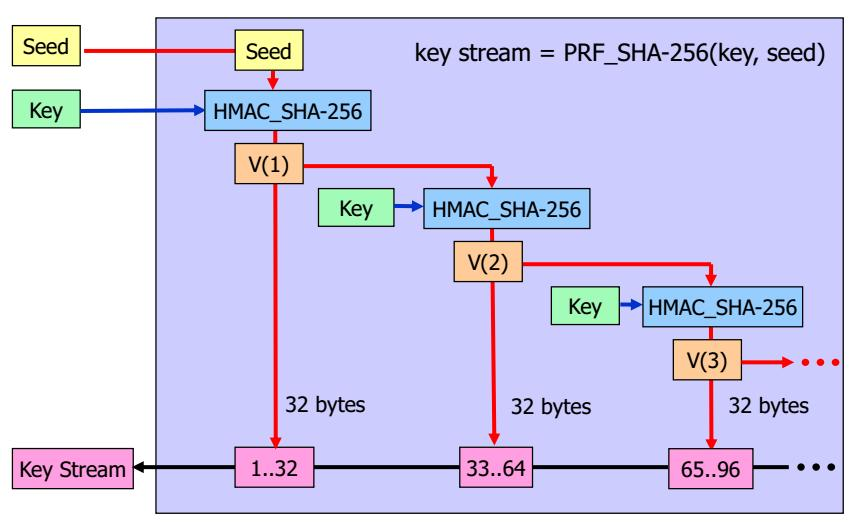
\includegraphics[width=0.7\linewidth]{images/hmac_prf}
\caption{HMAC PRF}
\label{fig:hmacprf}
\end{figure}


\subsubsection{DRBG: Deterministic Random Bit Generator}
Möchte man einen Key mit einer Schlüsselstärke ''X'' generieren, muss ein DRBG mindestens ''X'' Bits +  $\frac{X}{2}$ Bits für die Random Nonce liefern. Ein DRBG hat mehrere Inputs:
\begin{description}
	\item[Seed]	Das ''Kaffeepulver'' aus eineren wahren Zufallsquelle
	\item[Instantiate] Wie Stark soll die Sicherheit sein: (112Bit), (128Bit), 192Bit, 256Bit
	\item[Entropy Input] Entropy with size at least equal to security strength
	\item[Nonce] \hfill 
	\begin{itemize} 
		\item Entropy with size at least equal to 0.5 * security strength
		\item Counter with repetition rate at least equal to 0.5 * security strength
	\end{itemize}
	\item[Personalization String]  \hfill \\
	Application Identifiers, Device Serial Numbers, User IDs, etc. (Optional, can be an empty string)
	\item[Additional Input] Any other private or public input (Optional, can be empty)
\end{description}
\begin{figure}[h]
\centering
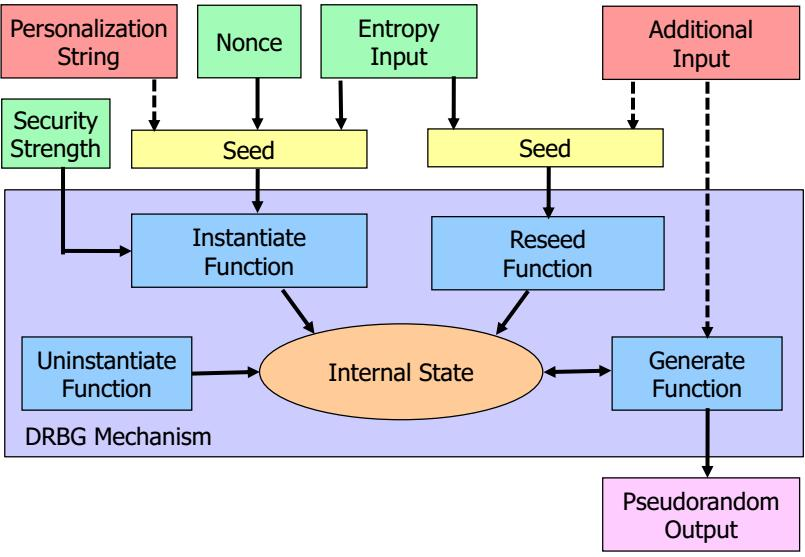
\includegraphics[width=0.5\linewidth]{images/drbg}
\caption{DRBG}
\label{fig:drbg}
\end{figure}

\subsection{Echte Random Generatoren}
Bei echten Random Generatoren zieht man die zufälligen Zahlen meist aus physikalischen Prozessen. Am besten ist, wenn man mehrere Quellen miteinander kombiniert.
\begin{itemize}
	\item Quantenquellen (die beste Quelle)
	\item Thermisches Rauschen 
	\item Radioaktiver Zerfall
	\item Intel RDRAND (gut und sehr schnell, sollte mit anderen Quellen vermischt werden, da evtl. die NSA ihre Finger im Spiel hat)
	\item Key Stroke Timing (kleine Entropie)
	\item Mouse Movements Coordinates (grosse Entropie)
	\item Soundcard Input Noise (Gefahr von Gesamtausfall)
	\item Air Turbulence in Disk Drives (Veraltet, da SSD)
	\item Network Packet Arrival Times (eher verpönt, da manipulierbar)
\end{itemize}


\section{Link Layer Security}

\subsection{WPA: Wi-Fi Protected Access (802.11i)}
Der Client (Supplicant) stellt eine Anfrage über \gls{eapol} an eine Access Point oder LAN Switch (Authenticator). Dieser überprüft beim einem Radius Server (Authentication Server) über EAP RADIUS, ob die Anfrage valide ist.

\subsection{Secure Device Identity (IEEE 802.1AR - DevID)}
Während der Herstellung wird eine IDevID (Initial Device Identifier) sowie ein X509 Zertifikat direkt auf die Hardware (DevID Module) geschrieben. Das DevID Modul verfügt zusätzlich über einen starken \gls{rng}  und implementiert starke asymetrische Algorithmen (2048 RSA oder 256 ECDSA) sowie eine Hash Funktion (SHA-256). Auf dem DevID Module kann eine LDevID (Local Significant Device Identifier) hinterlegt werden.

\subsection{MACsec: Media Access Layer Security (IEEE 802.1AE)}\label{sec:macsec-media-access-layer-security-ieee-8021ae}
MACsec erlaubt \textbf{sichere E2E Verbindungen} über Ethernet zwischen direkt verbunden Clients. MACsec nutzt \textbf{AES-GCM-128} für die Verschlüsselung. Seit 2011 kann auch AES-GCM-256 verwendet werden. Eine neuer PAE muss den pre-shared CAK des CA-Verbund kennen
\begin{description}
	\item[PAE: Port Access Entity] Ein Client (SecY). Jede PAE hat einen Secure Channel zu allen anderen Mitglieder in der CA. Jeder PAE muss den CAK der CA besitzen.
	\item[CA: Connectivity Association] Verbund von mehrere Clients auf L2 mit einem gemeinsamen Netzwerkschlüssel
	\item[CAK: Connectivity Association Key] Statischer Schlüssel die jede PAE/SecY in der CA kennen muss. Diese müssen manuell verteilt werden. (Im Heim-WLAN auch als \gls{psk} bezeichnet.) Der CAK verschlüsselt die Control Plane. Der CAK ist somit das Shared Secred eines CA Verbund.
	\item[CKN: CAK Name] Netzwerk Identifier (am besten Human-Readable; WLAN: SSID)
	\item[SAK: SA Key] Secure Association Key (Session Key). Es wird für jeden Client ein SAK benötigt. Jeder SAK wird vom CAK abgeleitet. (Hash über den CAK OR-verknüpft mit einem Random Wert des Key Servers). Der Keyserver ist entweder ein PAE oder der Access Point. Der SAK verschlüsselt die Data Plane.
	\item[SC: Secure Channel] Jede SC umfasst eine Reihe von SA mit unterschiedlichen SAK's. Jeder SC ist unidirectional. 
	\item[SA: Secure Association] Eine Verbindung zwischen zwei Clients. Es gibt mehrere SA's innerhalb einer SC. Jede SA hat seinen eigenen SAK. Es dürfen mehrere Associations innerhalb von einem SA in eine Richtung koexistieren, damit die SAK's (der SA) unterbruchsfrei ausgetauscht werden können.  Die SA's haben dann nur eine begrenzte Lebensdauer, während die SC's als Grundelemente einer CA immer existieren. 
\end{description}

\begin{figure}[h]
	\centering
	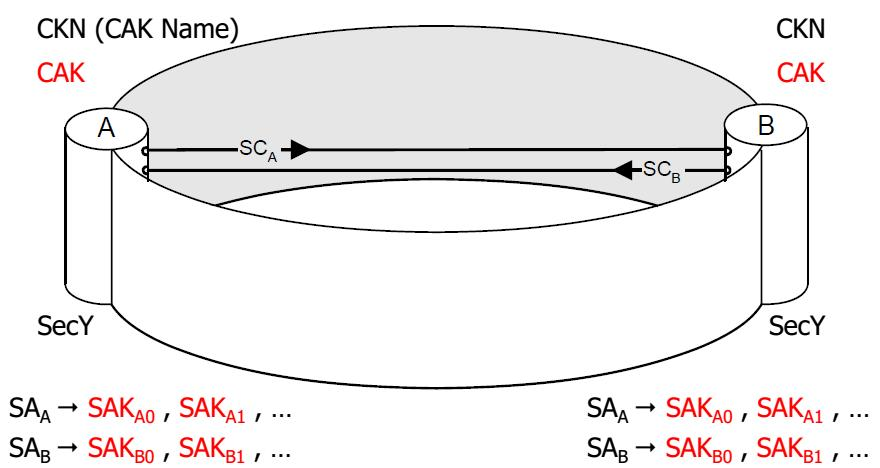
\includegraphics[width=0.6\linewidth]{images/macsec_sc_sa}
	\caption{MACsec Secure Channel}
	\label{fig:macsecscsa}
\end{figure}


\subsubsection{MKA: MACsec Key Agreement Protocol}
Dank dem 802.1X MACsec Key Agreement (MKA) Protokoll
können die SAK's mittels eines Key Servers dynamisch generiert und an alle Teilnehmer verteilt werden. Damit ist ein periodisches Rekeying möglich.

\subsubsection{SAI: Secure Association Identifier}
Der Secure Association Identifier dient als ID für eine SA. Er besteht aus einem System Identifier, einem Port Identifier und einer Association Number. Die 2 Bit lange Association Number erlaubt es, dass währende dem Rekeying zwei verschiedenen SAK's koexistieren können.

\subsubsection{MACsec Frames}
\begin{description}
	\item[MPDU: MACsec Protocol Data Unit] Beinhaltet SecTag, Payload und ICV. Die PDU werden mit \gls{eapol} verteilt.
	\item[MSDU: MAC Service Data Unit] Payload
	\item[ICV: Integrity Check Value] Ist der Authentication Tag der aus AES GCM/AES GMAC resultiert.
	\item[SA, DA] Source und Destination MAC Adresse im Klartext
	\item[SecTag] Security Tag vor dem Payload  im Klatext (Ethertype 0x88E5)
	\begin{itemize}
		\item Das E Bit definiert ob verschlüsselt wird
	\end{itemize}
	\item[FCS: Frame Check Sequence] 
\end{description}
\begin{figure}[h]
\centering
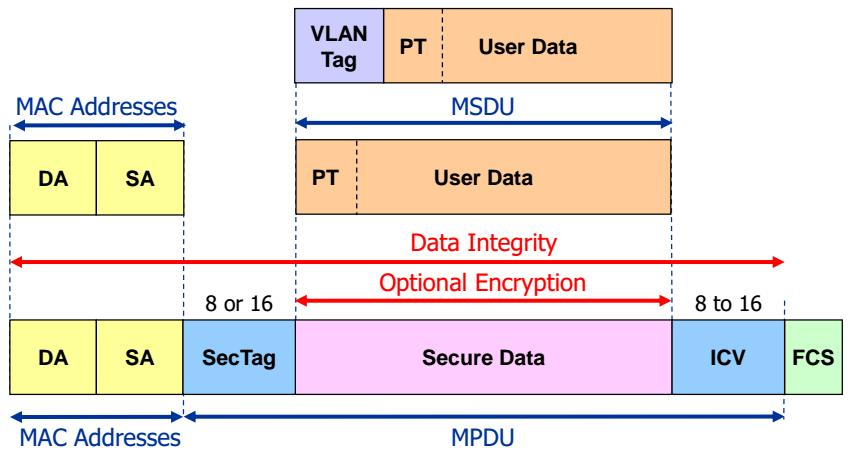
\includegraphics[width=0.5\linewidth]{images/macsec_frame_format}
\caption{MACSec Frame}
\label{fig:macsecframeformat}
\end{figure}


\section{VPN: Virtual Private Network}
Mittels VPN kann ein sogenannter Road Warrior (Client) von einem beliebigen Punkt auf der Erde via Internet auf sein heimatliches Firmennetz zugreifen. Bei IPsec geschieht das über einen verschlüsselten Tunnel, der zwischen Remote Access Client und dem Security Gateway des Heimatnetzes aufgebaut wird. Die Authentisierung der beiden Tunnelpunkte wird über ein X.509 Zertifikate bzw. Benutzername/Passwort bewerkstelligt. Es gibt verschiedene Varianten von VPNs wobei wir den Schwerpunkt auf IPsec legen. Aktuell wird IPsec mit IKEv2 empfohlen.

\subsection{Terminologie}
\begin{description}
	\item[VPN] Das konventionelle VPN bezeichnet einzig eine logische Trennung innerhalb einer physischen Leitung. 
	\item[SSL VPN] Erlaubt verschlüsselten Fernzugriff auf Unternehmensanwendungen um auf entfernte Ressourcen gesichert zuzugreifen.
\end{description}

\begin{figure}[ht!]
	\centering
	\begin{minipage}[t]{0.4\textwidth}
		\centering
		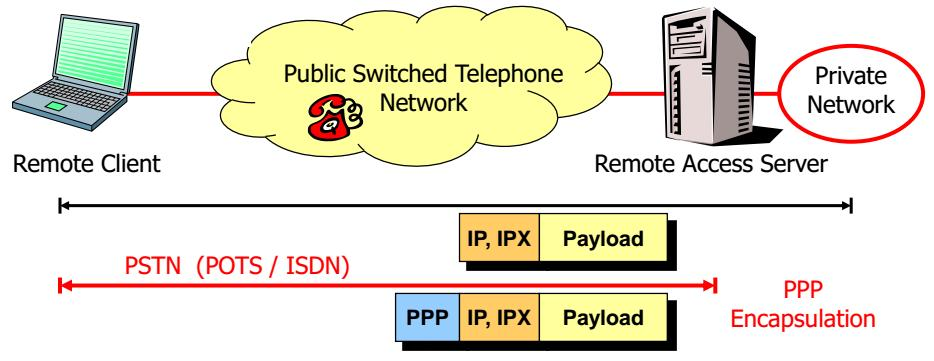
\includegraphics[width=\linewidth]{images/ppp_remote_access}
		\caption{PPP Remote Access über Einwählleitung}
		\label{fig:pppremoteaccess}
	\end{minipage}
	\begin{minipage}[t]{0.4\textwidth}
		\centering
		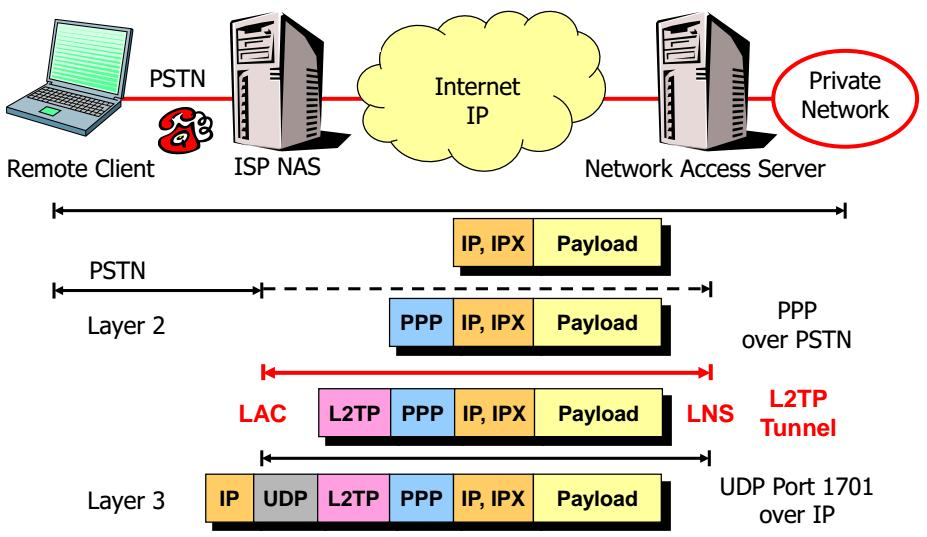
\includegraphics[width=\linewidth]{images/l2tp_remote_access}
		\caption{L2TP Remote Access}
		\label{fig:l2tpremoteaccess}
	\end{minipage}
	
	\begin{minipage}[t]{0.4\textwidth}
		\centering
		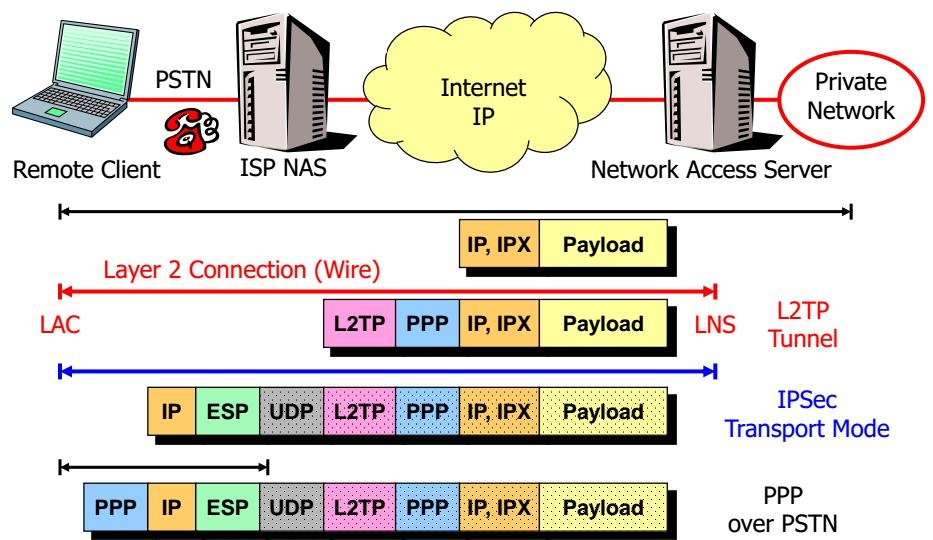
\includegraphics[width=\linewidth]{images/l2tp_ipsec_remote_access}
		\caption{L2TP über IPsec}
		\label{fig:l2tpipsecremoteaccess}
	\end{minipage}
	\begin{minipage}[t]{0.4\textwidth}
		\centering
		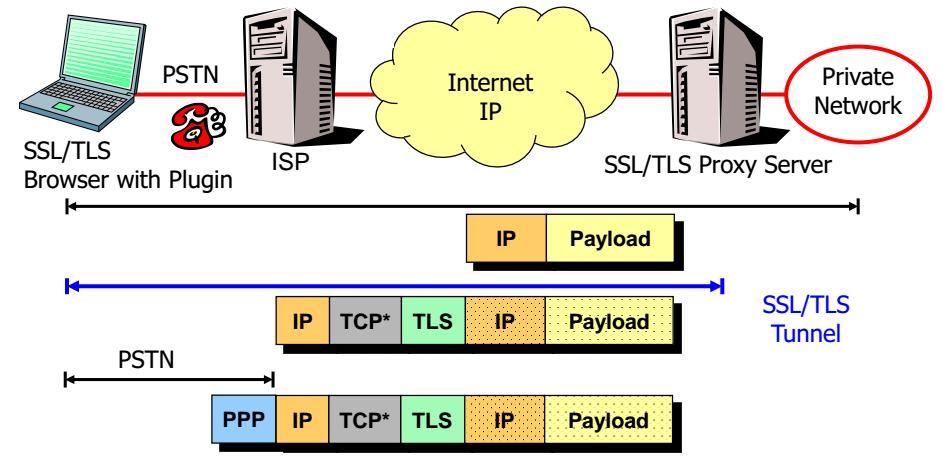
\includegraphics[width=\linewidth]{images/l4_tls_tunnel}
		\caption{VPN als TLS Layer 4 Tunnel}
		\label{fig:l4tlstunnel}
	\end{minipage}
\end{figure}

\subsection{MPLS-VPN: Multi-Protocol Label Switching}
Bei MPLS muss beachtet werden, dass nichts verschlüsselt wird. Ein ISP möchte mit MPLS nur eine logische Trennung der Kunden durchführen.


\clearpage

\subsection{IPsec: Internet Protocol Security}\label{sec:ipsec-internet-protocol-security}
\begin{figure}[h]
\centering
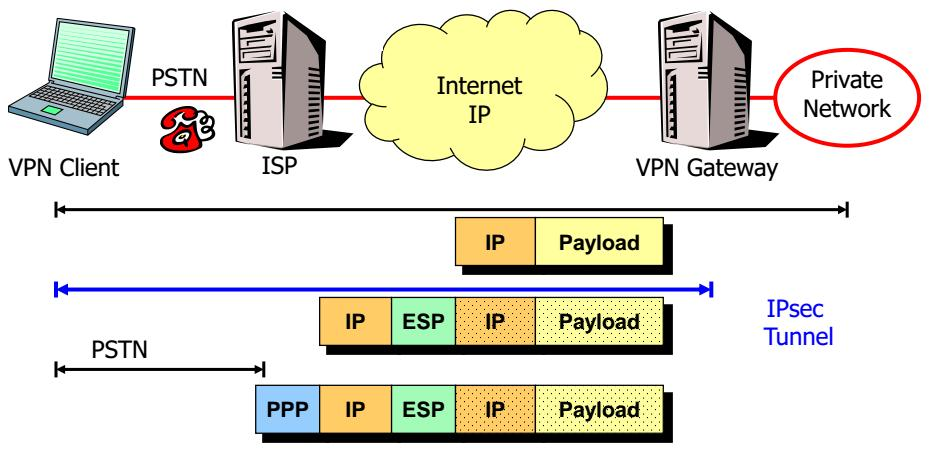
\includegraphics[width=0.5\linewidth]{images/ipsec_remote_access}
\caption{IPsec Remote Access}
\label{fig:ipsecremoteaccess}
\end{figure}

\begin{itemize}
	\item IPsec ist eine Protokoll Suite (Bausatz). Dass heisst, man kann die einzelnen Teile miteinander kombinieren.
	\item IPsec definiert die Vorgehensweise für die Datenintegrität, die Vertraulichkeit der Inhalte sowie die Verwaltung der kryptografischen Schlüssel. Es besteht aus folgenden Bausteinen
	\begin{description}
		\item[AH] Authentication Header
		\item[ESP] Encapsulating Security Payload
		\item[SA] Security Association
		\item[SPI] Security Parameter Index (32Bit): Identifier der SA
		\item[IKE] Internet Key Exchange (Siehe Sektion \ref{sec:ike})
	\end{description}
	\item Zu Beginn der Kommunikation wird zwischen den Clients das benutzte Verfahren ausgehandelt. IPsec unterscheidet je nach Art der Verschlüsselung zwischen dem AH basierten Transportmodus und dem ESP basierten Tunnelmodus.
	\item Path MTU Discovery muss funktionieren. Somit kann IPsec den korrekten Overhead von der MTU abziehen und sendet so nie eine zu grosse MTU, die dann auf dem Weg gedropt wird. (Bsp. Ping funktioniert, Grösserer Download nicht $\rightarrow$ MTU Einstellungen prüfen, oder MTU manuell setzen.)
	\item IPsec hat seine Stärke besonders bei der Performance.
	\item Der äussere IP Header dient dem Routing zwischen den beiden VPN Gateways, Der innere IP Header beinhaltet die IP Adressen der beiden Clients.
\end{itemize}

\clearpage

\subsubsection{AH: Authentication Header}
\begin{itemize}
	\item Meist als zusätzlicher IP-Header verpackt: IP Protokoll Nr. 51
	\item Es ist für die Authentizität und Integrität der übertragenen Pakete zuständig authentifiziert den Server
	\item Es schützt gegen Replay Attacken
	\item Der AH schützt das komplette Paket. (Ausgenommen sind Felder die auf dem Weg verändert werden. z.B TTL, ToS, Fragment Offset, IP Header Checksum)
	\item Ein Nachteil von AH ist, dass es inkompatibel mit NAT ist, da NAT Teile des IP Headers ändert, die gemäss AH nicht verändert werden dürfen.
\end{itemize}


\paragraph{Transport Mode} \hfill
\begin{figure}[h]
\centering
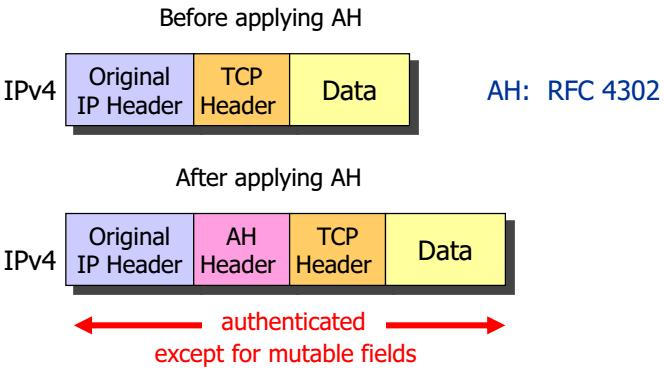
\includegraphics[width=0.5\linewidth]{images/ipsec_ah_header}
\caption{Transport Mode}
\label{fig:ipsecahheader}
\end{figure}

\paragraph{Tunnel Mode} \hfill
\begin{figure}[h!]
	\centering
	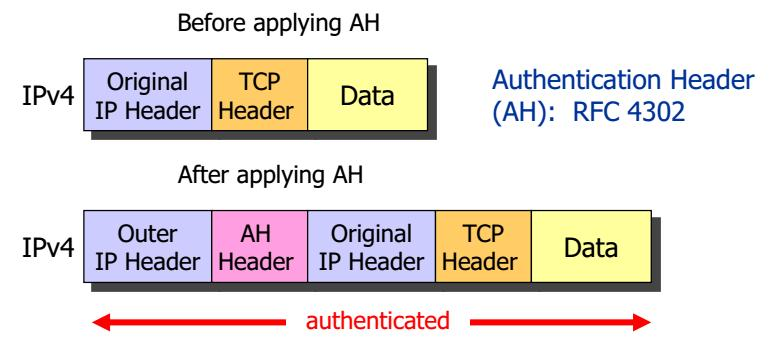
\includegraphics[width=0.7\linewidth]{images/ipsec_ah_transport}
	\caption{Tunnel Mode}
	\label{fig:ipsecahtransport}
\end{figure}


\subsubsection{ESP: Encapsulating Security Payload}
\begin{itemize}
	\item Ein zusätzlicher Header und Trailer um den Layer 4 Payload.
	\item IP Protokoll Nr 50 (Kein Port $\rightarrow$ Kein NAT, ausser ESP in UDP gepackt)
	\item Ist für die Sicherstellung der Authentizität, Integrität und Vertraulichkeit von IP Paketen zuständig
	\item Die Nutzdaten, Padding, Pad Lenght und Next Header werden verschlüsselt
	\item Im Unterschied zum AH wird der Kopf des IP-Paketes vom \gls{icv} nicht authentifiziert.
\end{itemize}
\paragraph{Transport Mode}\hfill
\begin{figure}[h!]
\centering
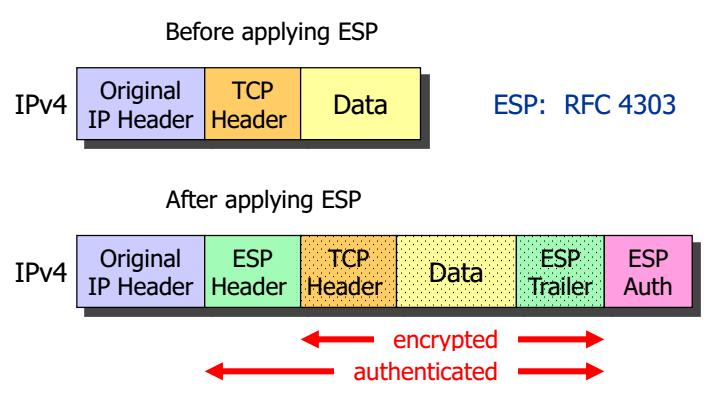
\includegraphics[width=0.5\linewidth]{images/ipsec_esp}
\caption{Transport Mode}
\label{fig:ipsecesp}
\end{figure}

\paragraph{Tunnel Mode}\hfill
\begin{figure}[h!]
	\centering
	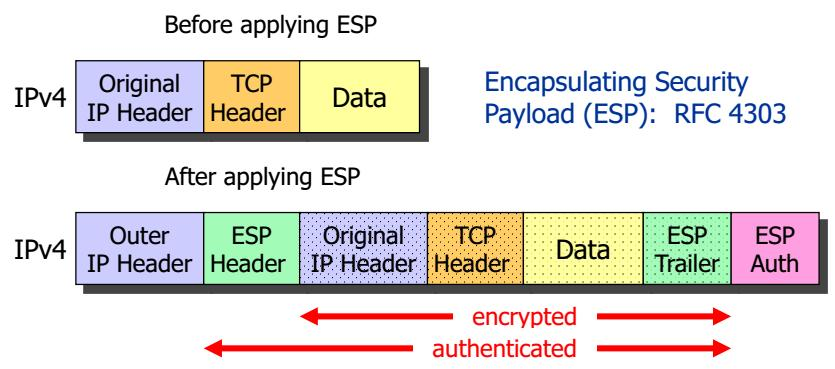
\includegraphics[width=0.7\linewidth]{images/ipsec_esp_tunnel}
	\caption{Tunnel Mode}
	\label{fig:ipsecesptunnel}
\end{figure}


\paragraph{NAT} \hfill \\
Mit der NAT Traversal Extension werden ESP Pakete in UDP verpackt, welche dann problemlos von NAT gemappt werden könnnen. Zusätzlich werden die Daten neu an Port 4500 gesendet, damit alte NAT-Router kein IP-Basiertes Traversal machen. Der Grund dafür ist, dass ESP ein eigenständiges L3 IP Protokoll (50) ist und somit keine Ports besitzt.
\begin{figure}[h]
\centering
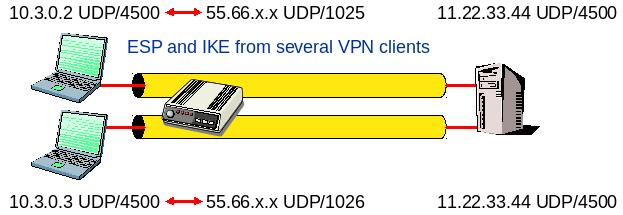
\includegraphics[width=0.5\linewidth]{images/ipsec_nat}
\caption{IPsec NAT}
\label{fig:ipsecnat}
\end{figure}

\subsection{StrongSwan}
Bei der Konfiguration von StrongSwan muss beachtet werden dass \textbf{left} die \textbf{lokale Domäne} und \textbf{right} für den \textbf{Remote} steht. 
\begin{description}
	\item[/etc/ipsec.d/cacerts] CA Zertifikate
	\item[/etc/ipsec.d/certs] User Zertifikate
	\item[/etc/ipsec.d/private] User Keys
	\item[/etc/ipsec.secrets] : ECDSA userKey.pem "your\_secrete\_pw"
\end{description}

\begin{lstlisting}[caption=/etc/ipsec.conf]
conn %default  
	leftcert=loginCert.pem // Cert das an die Gegenstelle gesendet wird
	// leftid = Per default distinguished name aus Cert

conn gateway-net 
	also=gateway // reuse content of "gateway" connection
	rightsubnet= 10.5.0.0/16

conn gateway 
	right= 152.96.31.50 // ip adresse der Gegenstelle
	rightid=intsec.hsr.ch 
	auto=add
	
ca hsr 
	cacert=hsrCert.pem
	ocspuri=http://intsec.hsr.ch:8880
	auto=add
\end{lstlisting}

\begin{figure}[h]
\centering
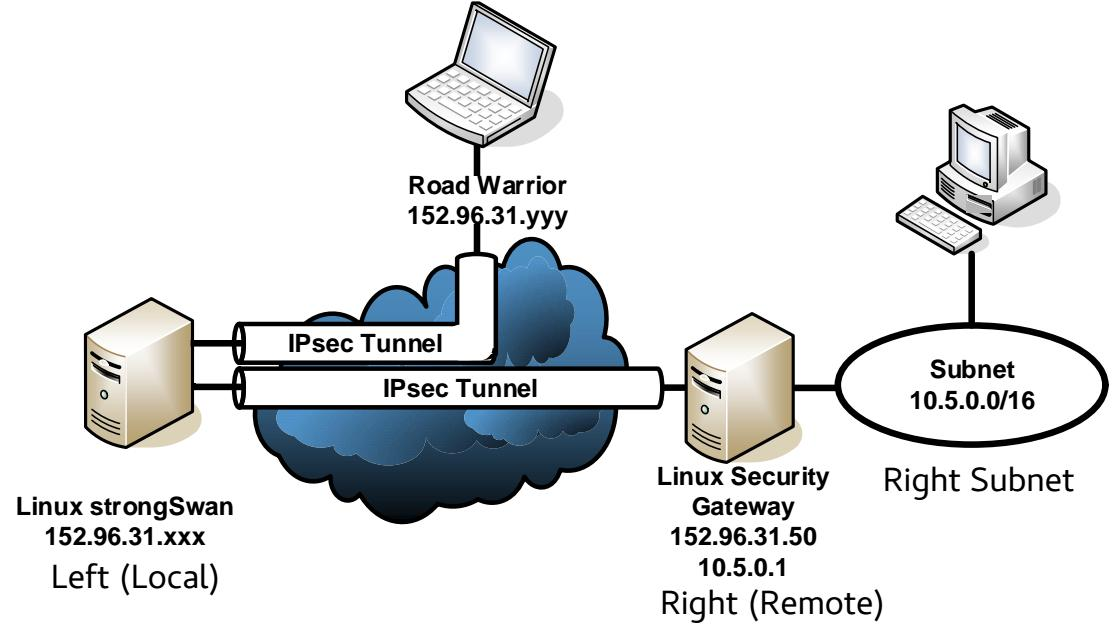
\includegraphics[width=0.4\linewidth]{images/ipsec_aufbau}
\caption{strongSwan Üubungs Aufbau}
\label{fig:ipsecaufbau}
\end{figure}

\subsubsection{Beispiel}
Für einen fixen Tunnel zwischen zwei Netzwerken (auf den Routern \lstinline|deviceA| und \lstinline|deviceB|)

\paragraph{deviceA} \hfill \\
\begin{lstlisting}
conn %default
	ikelifetime=60m
	keylife=20m
	rekeymargin=3m
	keyingtries=1
	authby=secret
	keyexchange=ikev2
	mobike=no

conn net-net
	left=deviceA.hsr.ch
	leftsubnet=192.168.1.0/24
	leftid=@deviceA.hsr.ch
	leftfirewall=yes
	lefthostaccess=yes
	right=deviceB.hsr.ch
	rightsubnet=192.168.2.0/24
	rightid=@deviceB.hsr.ch
	auto=route
\end{lstlisting}

\paragraph{deviceB} \hfill \\
\begin{lstlisting}
conn %default
	ikelifetime=60m
	keylife=20m
	rekeymargin=3m
	keyingtries=1
	authby=secret
	keyexchange=ikev2
	mobike=no

conn net-net
	left=deviceB.hsr.ch
	leftsubnet=192.168.2.0/24
	leftid=@deviceB.hsr.ch
	leftfirewall=yes
	lefthostaccess=yes
	right=deviceA.hsr.ch
	rightsubnet=192.168.1.0/24
	rightid=@deviceA.hsr.ch
	auto=route
\end{lstlisting}





\section{IKE: Internet Key Exchange}\label{sec:ike}
Für den Verbindungsaufbau einer IPsec Verbindung ist das sogenannte Internet Key Exchange Protokoll zuständig. Seit 2005 kann das verbesserte IKEv2 verwendet werden. 4 Jahre später war Windows 7 die erste kommerziell verfügbare Implementierung des Standards.
\begin{itemize}
	\item Das \gls{ike} Protokoll ist für den Aufbau einer \gls{sa} zuständig. Eine SA muss \textbf{einmal für jede Richtung (unidirektionl)} ausgehandelt werden.
	\item Das Protokoll dient der Verwaltung und zum Austausch der Schlüssel in IPsec. Zusätzlich bietet es ein standardisiertes Verfahren für die Authentifizierung von Kommunikationsparter sowie zur Erzeugung von gemeinsam genutzten Schlüsseln.
	\item UDP Port 500 (Socketverbindung) / 4500 (Übertragung)
	\item Aktuell gibt es zwei Versionen von IKE: Version 1 arbeitet in zwei Phasen und Version 2 braucht viel weniger Meldungen für den Verbindungsaufbau. 
\end{itemize}

\subsection{Version 1}
\begin{itemize}
	\item ISAKMP\_SA handelt die Paramter für die IKE Übertragung selbst aus.
	\item Verwendet Pre-Shared Secrets oder Public Key
	\item Verwendet XAUTH zur erweiterten Authentisierung (Überträgt Passwort im Klartext)
	\item Ein Verbindungsaufbau zwischen zwei Endstations benötigt 15 Meldungen.
	\[
	12 = 6 (Phase 1) + 3 (Phase 2: Richtung A) + 3 (Phase 2: Richtung B)
	\]
\end{itemize}

\subsubsection{Ablauf}
In der Version 1 wird der IPsec Verbindungsaufbau in zwei Phasen eingeteilt:
\begin{enumerate}
	\item In einer ersten Phase baut IKE eine Verbindung mit relativ schwachen Sicherheitsmechanismen auf, die der Absicherung und Authentifizierung der weiteren Verwaltungsvorgänge dient. Nach der ersten Phase steht eine ISAKMP\_SA, welche bidirektional ist. Dieser Schritt benötigt 6 Pakete (ausser im Agressive Mode)
	\item In einer zweiten Phase wird das zu verwendende Sicherheitsprotokoll ausgehandelt und umgesetzt. Dazu wird der in der Phase 1 erstellte Tunnel verwendet. Für diese Phase werden für \textbf{jede Richtung} je 3 Pakete verwendet. Es resultiert eine ESP SA über welche dann die wirklichen Daten übertragen werden.
	\begin{itemize}
		\item Zuerst schlägt der Client seine unterstützten Cipher Suites vor
		\item Das Gateway antwortet dann mit seiner Auswahl
		\item In dieser Phase werden auch die DH Schlüssel generiert
	\end{itemize}
\end{enumerate}



\clearpage

\subsubsection{Phase 1: Modes}
In einer ersten Phase handelt IKE die Parameter für die ISAKMP\_SA aus. Dabei gibt es verschiedene Modes:
\begin{description}
	\item[Main Mode] Das Problem beim Main Mode ist die Performance. Zusätzlich besteht das Problem, dass ein MitM Angreifer den Session Key des DH Exchange abfangen kann, da die ersten 4 Pakete im \textbf{Klartext} übertragen werden. Das Zertifikat wird in den letzten beiden Paketen übertragen.
	\item[Main Mode mit Pre Shared Keys] Die ersten vier Pakete sind gleich wie im Main Mode. Zusätzlich wird das Password (\gls{psk}) in den Hash eingearbeitet. Dies verhindert einen MitM Angriff. Ebenfalls ist somit die Indentität verschlüsselt.
	\item[Agressive Mode mit Pre Shared Keys] Beim Aggressive Mode ist das Ziel möglichst schnell die Phase 1 abzuarbeiten. Man schickt deshalb mehr Informationen pro Paket. Das grosse Problem ist, dass der Hash unverschlüsselt übertragen werden. (beim 2. Paket)
\end{description}

\begin{figure}[ht!]
	\centering
	\begin{minipage}[t]{0.4\textwidth}
		\centering
		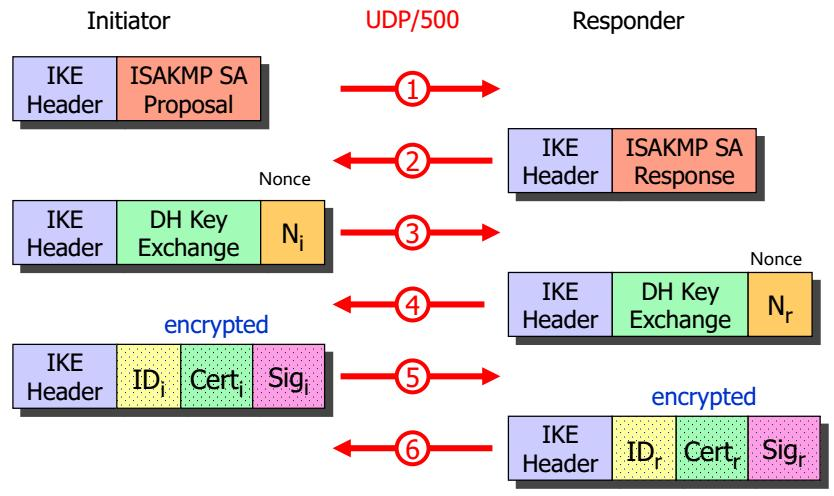
\includegraphics[width=\linewidth]{images/ike_v1_main_mode}
		\caption{IKE Main Mode}
		\label{fig:ikev1mainmode}
	\end{minipage}
	\begin{minipage}[t]{0.4\textwidth}
		\centering
		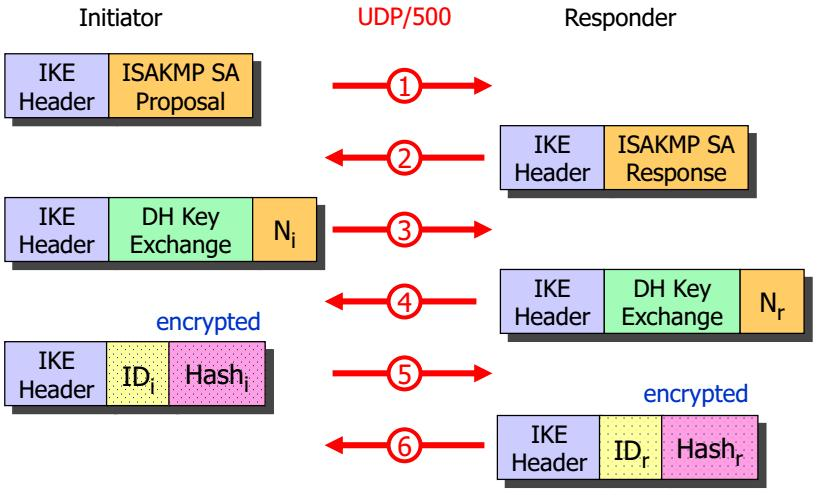
\includegraphics[width=\linewidth]{images/ike_v1_main_mode_presharedkeys}
		\caption{Main Mode mit Pre-Shared Keys}
		\label{fig:ikev1mainmodepresharedkeys}
	\end{minipage}
	\begin{minipage}[t]{0.4\textwidth}
		\centering
		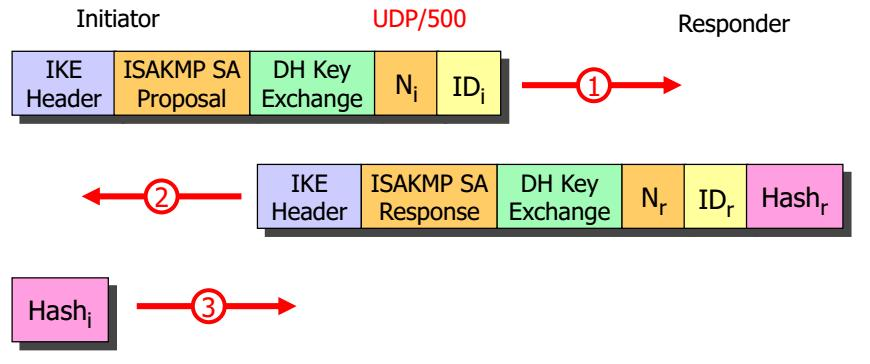
\includegraphics[width=\linewidth]{images/ike_v1_aggressive_mode_presharedkeys}
		\caption{Agressive Mode mit Pre-Shared Keys}
		\label{fig:ikev1aggressivemodepresharedkeys}
	\end{minipage}
\end{figure}


\subsubsection{Phase2: Quick Mode}
In der Phase zwei wird mit 3 weiteren Paketen die SA über den sicheren Kanal der in Phase 1 ISAKMP\_SA aufgebaut wurde, erstellt. Die ISAKMP ist \textbf{bidirektonal}. Die IPsec SA besteht aus zwei Traffic Selectors. Es gibt einen Traffic Selector für den Initiator und den Responder. Der Traffic Selektor definiert also eine Endstation. 

\clearpage

\subsection{Version 2}
\begin{itemize}
	\item IKEv2 verwendet standardmässig nur 1024Bit DH für den Schlüsselaustausch. 
	\item IKE SA ist das v2 Pendant zum ISAKMP\_SA unter v1
	\item IKE v2 ist komplett neu, bis auf den Port 500
	\item IKE v2 verfügt über die Möglichkeit Child SA zu erstellen. Dies wird besonders beim Re-Keying verwendet.
	\item Verwendet \gls{eap} zur erweiterten Authentisierung
	\item IKE v2 unterstütz Cookie Mechanismus gegen DoS Attacken (nicht aber gegen DDoS, da die Zombies die Cookies zurücksenden)
	\item Bei IKEv2 wurde auf einen präventiven Cookie-Austausch verzichtet (Es gibt selten Probleme mit DOS). Der Cookie Mechanismus kann jedoch manuell aktiviert werden. 
	\item Nur noch 4 anstatt den 9 Meldungen in V1
	\item Ein Verbindungsaufbau zwischen zwei Endstations benötigt 6 Meldungen:
	\[
	6 = \text{4 (je 2 für IKE\_SA und IKE\_AUTH: beinhaltet bereits eine Child SA!) + 2 (Child SA)}
	\]
\end{itemize}


\begin{figure}[ht!]
	\centering
	\begin{minipage}[t]{0.4\textwidth}
		\centering
		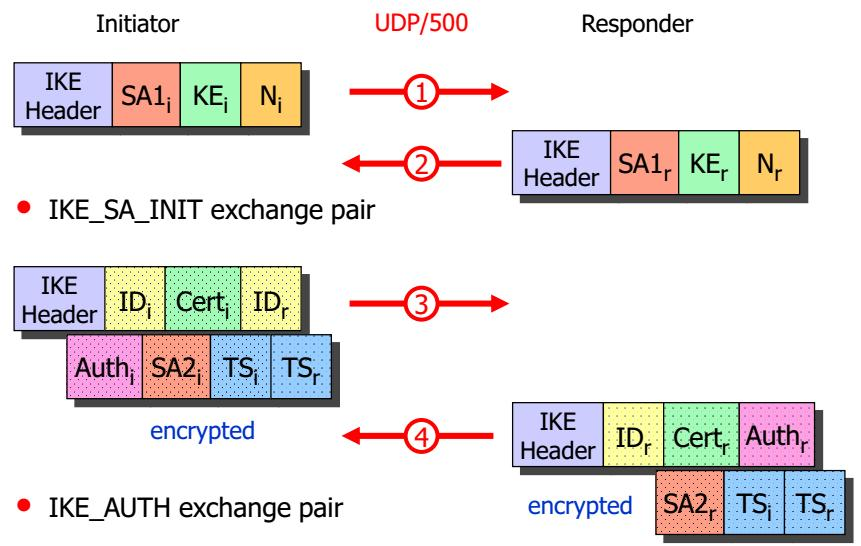
\includegraphics[width=\linewidth]{images/ike_v2}
		\caption{IKE V2: First Child SA}
		\label{fig:ikev2}
	\end{minipage}
	\begin{minipage}[t]{0.4\textwidth}
		\centering
		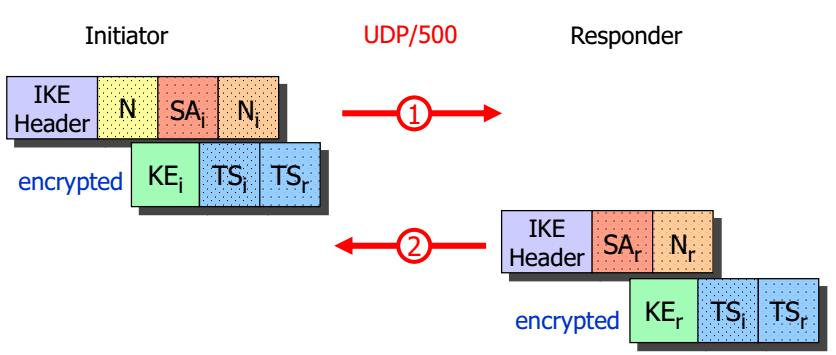
\includegraphics[width=\linewidth]{images/ike_v2_additional_sa}
		\caption{IKE V2: Additional Child SA}
		\label{fig:ikev2additionalsa}
	\end{minipage}
\end{figure}

\subsubsection{Ablauf}
\begin{itemize}
	\item IKE\_SA\_INIT Request und Response im Klartext
	\begin{itemize}
		\item Im SA Payload sind die ausgehandelten Cipher Suites sichtbar
	\end{itemize}
	\item IKE\_AUTH Request und Response (Erstellt SA zum Gateway)
	\item CREATE\_CHILD\_SA Request und Response (Erstellt SA vom Gateway ins Netz hinter dem Gateway)
\end{itemize}

\subsubsection{Narrowing}
Narrowing vereinfacht die Konfiguration von IKEv2 um ein Vielfaches. Beim Narrowing wird automatisch das kleinste Subnetz genommen.

\section{DNSSEC: DNS Security Extensions}

\subsection{DNS}
\begin{itemize}
	\item DNS basiert auf UDP und deshalb ohne erweiterten Sicherheitsmassnahmen (Source Port Randomization und Query ID Randomzation) einfach zu spoofen.
	\item Rekursive Auflösung: Bei der rekursiven DNS Server fragt der lokale Namensserver rekursiv alle benötigten externen Nameserver an, um die Adresse aufzulösen.
	\item Der Source Port ist im Standard nicht definiert. Der Destination Port von DNS ist immer 53
	\item Die QID (16 Bit Query ID) identifiziert einen DNS Request. Sie muss gleich wie die DNS Response Transaction ID sein.
	\item Query ID und Source Port müssen passen, damit ein DNS Server einen Request beantwortet.
\end{itemize}
\begin{figure}[ht!]
	\centering
	\begin{minipage}[t]{0.4\textwidth}
		\centering
		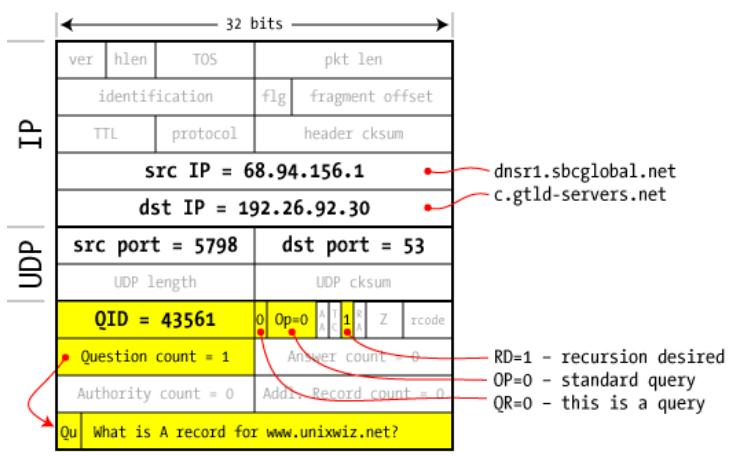
\includegraphics[width=\linewidth]{images/dns_request}
		\caption{DNS Request}
		\label{fig:dnsrequest}
	\end{minipage}
	\begin{minipage}[t]{0.4\textwidth}
		\centering
		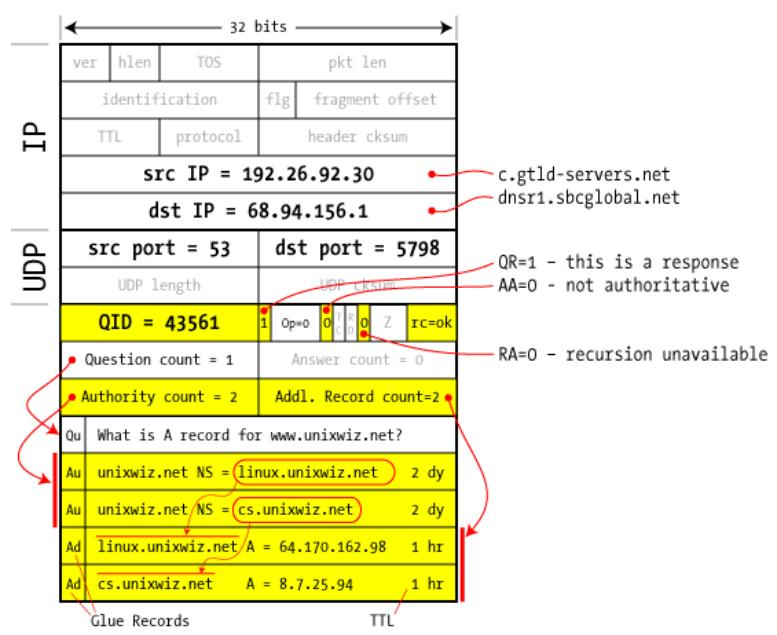
\includegraphics[width=\linewidth]{images/dns_response}
		\caption{DNS Response}
		\label{fig:dnsresponse}
	\end{minipage}
\end{figure}

\subsection{DNS Cache Poisoning}
Beim DNS Cache Poisoning versucht ein Angreifer die Query ID und den Source Port zu erraten und dabei eine schnellere Antwort zu liefer, als das dies der korrekte NS macht. Der erste DNS Response der beim Client NS ankommt, wird in den Cache geschrieben und alle weitere Anfragen laufen dann, im schlimmsten Fall über den NS des Angreifers. Hat er sein Ziel erreicht, kann er alle DNS Requests und MX Records für eine Zone manipulieren.

\clearpage

\subsection{DNSSEC Resource Records}
Mit DNSsec kann man sicher gehen, dass die zurückgelieferten DNS Records vertrauenswürdig sind. Dazu muss man einzig dem KSK der Root Zone vertrauen. Dieser muss im DNS Resolver hinterlegt werden.
\begin{description}
	\item[KSK: Key Signing Key (Flag=257)] langfristiger Schlüssel (2048Bit RSA). Mit dem KSK wird wird der ZSK signiert.
	\item[ZSK: Zone Signing Key (Flag=256)] Mit diesem werden alle Zone Records signiert. Dies wird bei jeder Generierung des Zonen-Files gemacht. (1024Bit RSA). Mit dem ZSK werden die DS Records der darunterliegenden Zonen signiert. (Root $\rightarrow$ Top Level $\rightarrow$ .. ) 
	\item[DS: Delegation Signer] 
	Der DS Record ist ein Hash über den Public Key (KSK) der darunter liegenden Zone. Erstellt man mit dem definierten Hash Algorithmus einen Hash über den Public Key kann dieser mit dem DS Record verglichen werden.
	\begin{lstlisting}[caption=DNSKEY]
	domain.ch. <time to live> IN DNSKEY <flag> 3 <algorithm>
	<base 64 public_key>; {id=<key tag id> (zks|ksk), size = <size>}
	\end{lstlisting}
	\item[RRset] Ein DNS Record Eintrag
	\item[DNSKEY] Ist ein Base64 codierter Public Key. Mit diesem wird die RRSIG Signatur wieder entschlüsselt. Daraus resultiert ein Hash. Mit dem gegebenen Hash Algorithmus muss der RRset (z.B A Record) gehashed werden. Sind die beiden Hashes gleich, kann dem DNS Server vertraut werden.
	\item[RRSIG: Resource Record Signature] Enthält die Signatur über ein RRset (z.B A Record, IPSECKEY Record oder DS Record)
	\begin{lstlisting}[caption=RRSIG]
	sub.domain.ch. <time to live> IN RRSIG <record_type> <algorithm> 3 <time to live>
	<valid from>
	<valid to>
	<key tag id> <parent domain>
	<signature>
	\end{lstlisting}
	\item[NSEC: Next Owner Name] Mit NSEC Records ist es möglich, alle Namen einer Zone aufzulisten. Man beginnt mit einer Anfrage nach einem NSEC Record bei einem bliebigen Namen und erhält damit den nächsten gültigen Namen. Seit Version 3 werden die Records mit gehashed. Man erhält also einen Hash zurück. Dieser kann nur noch mit einer Dictionary Attack geknackt werden.
\end{description}

\clearpage

\subsubsection{Ablauf: Chain of Trust}
\begin{enumerate}
	\item Die Zone \lstinline|switch.ch.| hat einen KSK (DNSKEY Eintrag) und einen ZSK (DNSKEY Eintrag). Der KSK signiert den ZSK. Der ZSK signiert alle weiteren DNS Records. Daraus resultieren RRSIG Einträge (Hashes)
	\item Die Zone \lstinline|.ch.|, hat ebenfalls einen KSK (DNSKEY Eintrag) und einen ZSK (DNSKEY Eintrag). Auch hier signiert der KSK den ZSK. Der ZSK signiert alle weiteren DNS Records. Auch hier resultieren RRSIG Einträge (Hashes)
	\item Damit dem KSK in der Zone \lstinline|switch.ch.| vertraut wird, muss diese manuell einen DS Eintrag in der darüberliegenden Zone (.ch.) erstellen. (Aufgabe des Sysadmin: Anfrage bei Top Level Zone)
	\item Dieser DS Eintrag wird vom ZSK der Zone ''.ch.'' signiert. Es resultiert wieder ein RRSIG Eintrag.
	\item Dies wird wiederholt bis am in der Root Zone angelangt ist.
\end{enumerate}

\begin{figure}[h!]
	\centering
	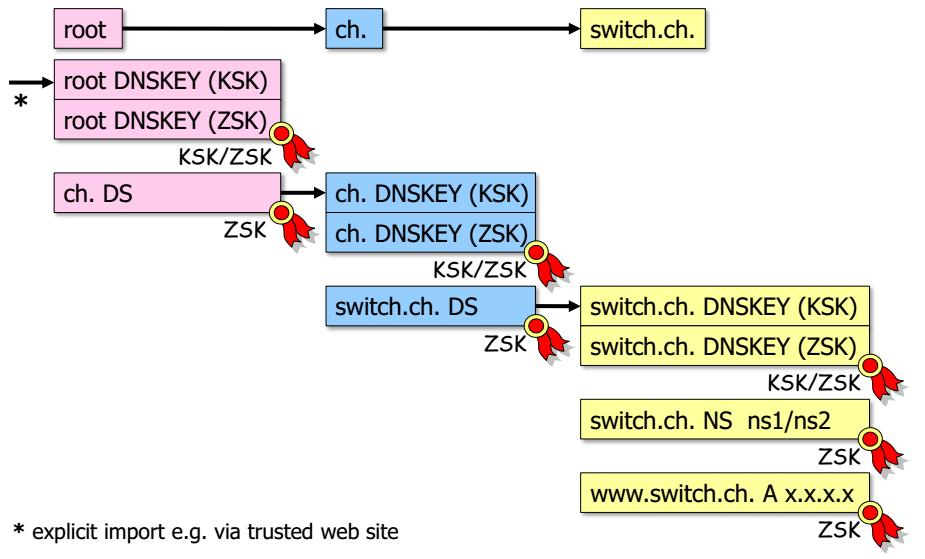
\includegraphics[width=0.9\linewidth]{images/dnssec_chainoftrust}
	\caption{DNSsec Chain of Trust}
	\label{fig:dnssecchainoftrust}
\end{figure}

\clearpage


\subsubsection{Verifikation}
Für die Verifikation muss der KSK der Root Zone, beim Client hinterlegt sein.
\begin{enumerate}
	\item Zuerst stellt der Client eine Anfrage für einen beliebigen Record an \lstinline|www.potaroo.net.|
	\item Die dafür zuständige Zone antwortet mit den geforderten Record und den RRSIG zu diesem Record. Um diesen RRSIG zu überprüfen wird der ZSK der Zone benötigt. 
	\item Der ZSK an sich muss aber auch überprüft werden. (Der könnte ja gefakt sein) Man überprüft deshalb den RRSIG des ZSK mit dem KSK der Zone
	\item Dem KSK kann aber auch nicht vertraut werden, solange er nicht verifiziert ist. Für den KSK existiert deshalb einen DS Eintrag in der darüberliegenden Zone. 
	\item Der DS Eintrag hat wiederum einen RRSIG Eintrag der mit dem ZSK der \lstinline|.net| Zone erstellt wurde.
	\item Die vorgehenden Schritte werden wiederholt, bis man bei der Root Zone ''.'' angekommen ist. Die Root Zone an sich wird mit dem beim Client hinterlegten KSK der Root Zone validiert.
\end{enumerate}


\begin{figure}[h]
	\centering
	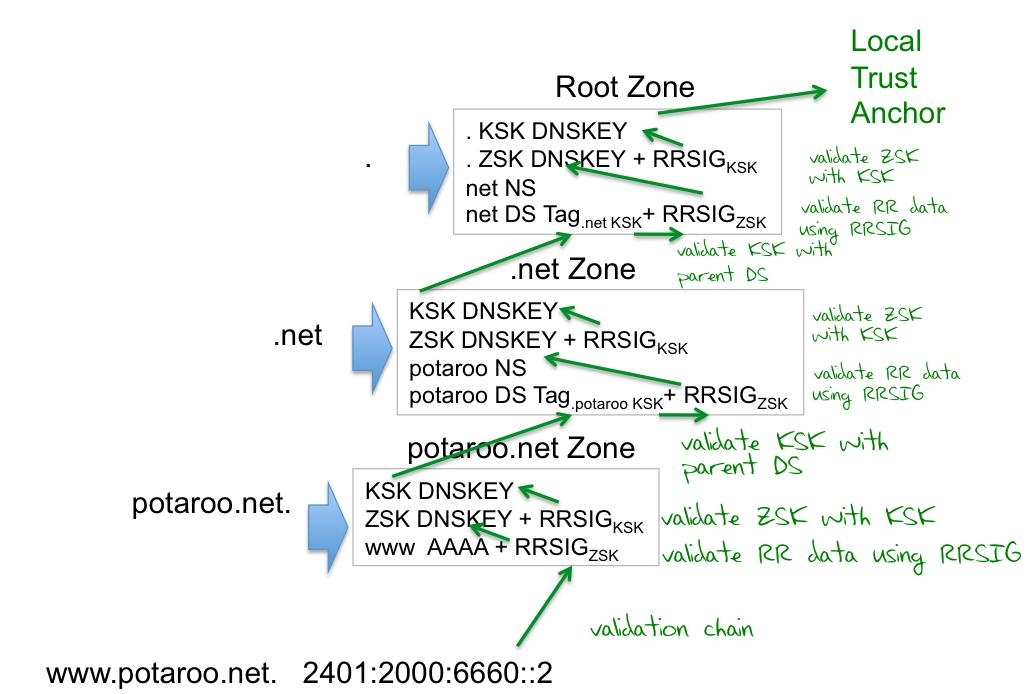
\includegraphics[width=0.9\linewidth]{images/dnssec_verification}
	\caption{DNSSec Verifikation}
	\label{fig:dnssecverification}
\end{figure}

\clearpage

\subsection{DANE: DNS-based Authentication of Named Entities}
Mit DANE können Clients den DNS Server anfragen, welche TLS Zertifikate als vertrauenenswürdig eingestuft werden können. DANE erweitert somit TLS, dass die verwendeten Zertifikate \textbf{ nicht unbemerkt ausgewechselt} werden können. Dazu werden X.509 Zertifikate mit DNS Einträgen verknüpft und per DNSSec als TLSA Resource Record gesichert. Ausserdem können Domaininhaber eigene Zertifikate ausstellen und so die Dienste der CA's umgehen.

\subsubsection{Funktionsweise}
\begin{enumerate}
	\item Ruft ein Client eine Webseite auf, möchte er sich sicher sein, dass der korrekte Server die Webinhalte ausliefert. Dazu prüft er das Zertifikat des Servers
	\item Anschliessend muss er sicherstellen, dass das Zertifikat von einer vertrauenswürdigen CA ausgestellt wurde. Da es sehr viele CA's gibt, kamen Zweifel an der Verlässlichkeit der CA's auf. Hier setzt DANE an
	\item Clients können mit können mit DANE bei den DNS Server nachfragen, welche Zertifikate sie als vertrauenswürdig einstufen können. Dies wird über einen neuen TLSA Resource Record gemacht. Dieser enthält das Zertifikat und dessen Finger oder public Key. 
\end{enumerate}


\subsubsection{TLSA Resource Record}
\begin{figure}[h]
\centering
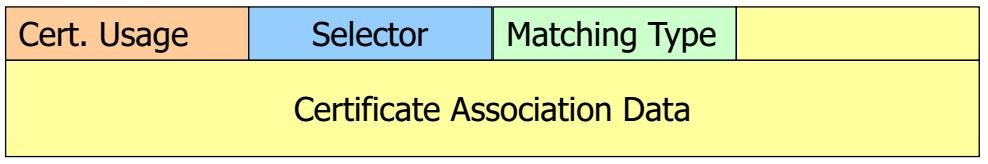
\includegraphics[width=0.7\linewidth]{images/tlsa_resource_record}
\caption{TLSA Resource Record}
\label{fig:tlsaresourcerecord}
\end{figure}

\begin{description}
	\item[Certificate Usage] \hfill
	\begin{itemize}
		\item 0 – CA Certificate Constraint
		\item 1 – Server Certificate Constraint
		\item 2 – Trust Anchor Assertion for Private CA
		\item 3 – Domain Issued Certificate
	\end{itemize}
	\item[Selector] \hfill
	\begin{itemize}
		\item 0 – Full Certificate
		\item 1 – Public Key Info (Public Key plus Key Type Information)
	\end{itemize}
	\item[Matching Type] \hfill
	\begin{itemize}
		\item 0 – Exact Match on Selected Content
		\item 1 – SHA-256 Hash of Selected Content
		\item 2 – SHA-512 Hash of Selected Content
	\end{itemize}
\end{description}


\section{VoIP Security}
Die SIP (Session Initiation Protocol) Kommunikation ist standardmässig unverschlüsselt. Ein SIP Client registriert sich normalerweise bei einem SIP Proxy. Dabei muss sich der Client beim Proxy authentifizieren. Der Proxy verbindet dann zwei VoIP Client miteinander. Hat der Proxy die Verbindung mit dem Endknoten hergestellt (Callee) wird ein RTP Kanal zwischen den beiden SIP Clients hergestellt. Bei der RTP muss die Confidientiality und Data Integrity sichergestellt werden. Um eine ersten Schutz zu implementieren, stellt man die VoIP Phones in ein eigenes VLAN. Dies bietet aber nur einen minimalen Schutz, da es immer noch möglich ist, einen VLAN Tag zu faken. 

\begin{figure}[h]
\centering
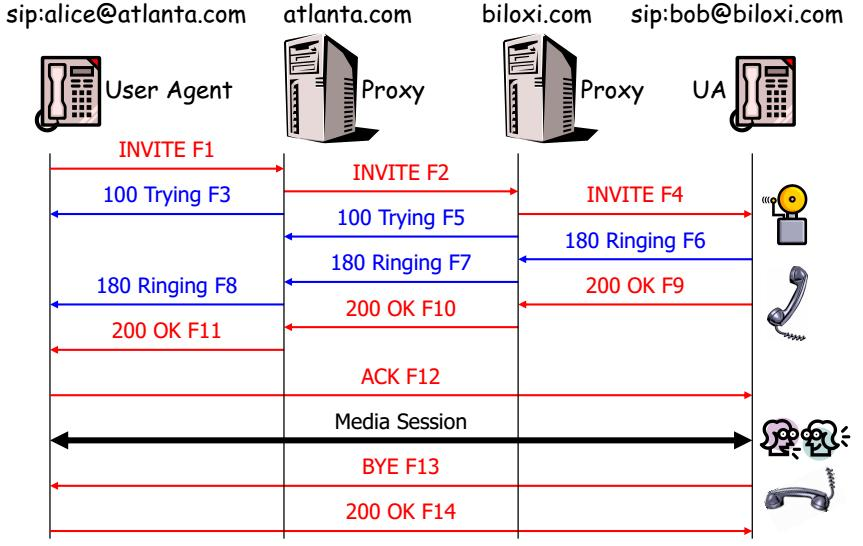
\includegraphics[width=0.7\linewidth]{images/sip_connection}
\caption{SIP Verbindung}
\label{fig:sipconnection}
\end{figure}

\subsection{SDES: Session Description Protocol Security Descriptions}
SDES ist ein Verfahren um Schlüssel via SIP auszutauschen. SDES überträgt die Schlüssel im Klartext. Aus diesem Grund sollte die Verbindung zum Proxy mit SIPS verschlüsselt sein und man sollte dem Proxy trauen können.

\clearpage

\subsection{ZRTP: Phil Zimmermann RTP}
ZRTP wurde von Phil Zimmermann (PGP) entwickelt. Sobald die Verbindung über den Proxy aufgebaut wurde, handeln die beiden Clients über RTP einen Diffie Hellman Schlüssel aus. Die ausgehandelten Keys werden nach dem Verbindungsaufbau mit einer Prüfsumme (4 Zeichen = Base32 Encoding der 20 MSB des 32 Bit langen \textbf{Short Authentication String (SAS)}) verifiziert. Somit kann sichergestellt werden, dass kein MitM auf der Leitung sitzt, da dann verschiedene SAS angezeigt werden.

\subsection{SRTP: Secure Real Time Protocol}
Bei SRTP wird der RTP Payload verschlüsselt und der Header inkl. Payload gehashed. Standardmässig wird mit AES-CTR (Stream Cipher) mit der Stärke von 128Bit verschlüsselt. Der Vorteil des Stream Ciphers ist, dass die Payload nicht grösser wird (kein Padding). Die Sequenznummer wird als Counter bei der Verschlüsselung verwendet. Anhand des Tags erkennt man ob ein SRTP Paket verschlüsselt ist.
\begin{figure}[h]
\centering
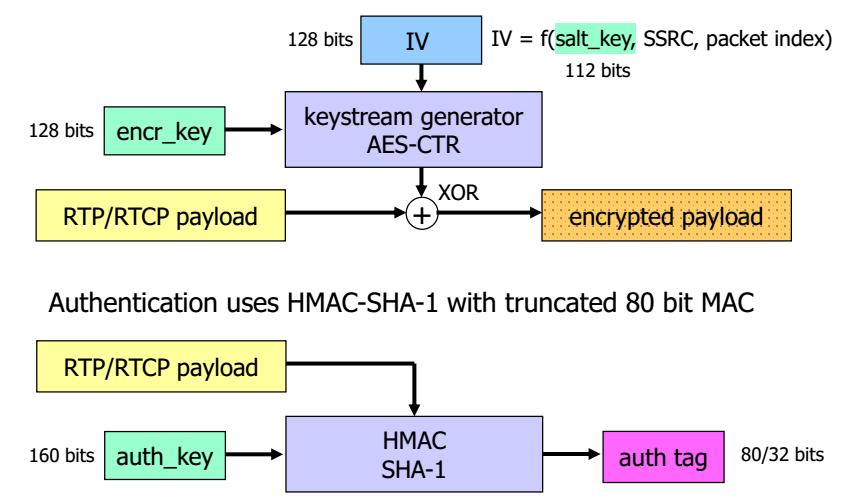
\includegraphics[width=0.5\linewidth]{images/srtp}
\caption{SRTP Encryption und Authentication mit AES CTR rsp. SHA-1}
\label{fig:srtp}
\end{figure}

\subsection{Session Key Derivation}
Zwischen den zwei Stationen muss einzig der Master Key übermittelt werden. 

\begin{figure}[h]
\centering
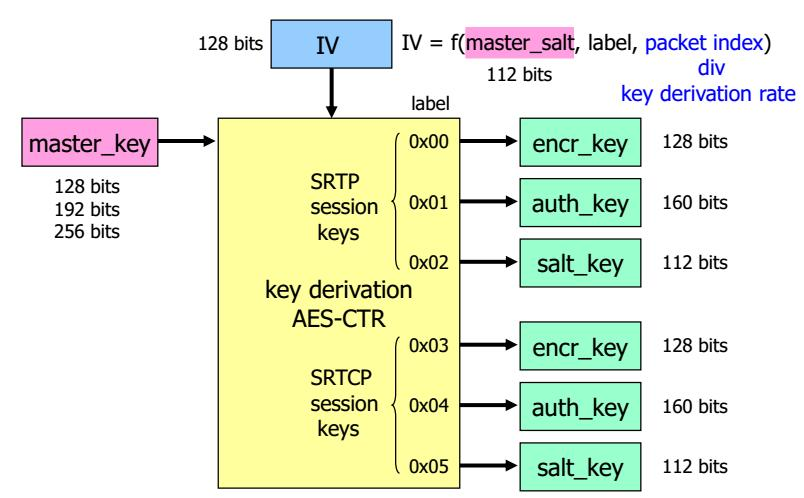
\includegraphics[width=0.5\linewidth]{images/srtp_key_derivation}
\caption{SRTP Key Derivation}
\label{fig:srtpkeyderivation}
\end{figure}

\subsection{SIPS: Session Initiation Protocol Secure}
SDP (Session Description Protocol) ist für die Übermittlung des Master Keys zuständig. Um SDP zu schützen wird SIPS verwendet. SIPS erstellt TLS Verbindungen zwischen SIP Caller und Proxy, Proxy und Proxy und Proxy zu SIP Callee. (Hop to Hop) Das Problem ist, wenn jemand Zugriff auf den Proxy Server hat, (Staat oder Hacker) kann der Master Key gesnifft werden, da die TLS Verbindung nicht E2E ist.

\begin{lstlisting}[caption=Unverschlüsselte SDP Master Key Übertragung (crypto)]
v=0
o=jdoe 2890844526 2890842807 IN IP4 10.47.16.5
s=SDP Seminar
i=A Seminar on the session description protocol
u=http://www.example.com/seminars/sdp.pdf
e=j.doe@example.com (Jane Doe)
c=IN IP4 161.44.17.12/127
t=2873397496 2873404696
m=video 51372 RTP/SAVP 31
a=crypto:1 AES_CM_128_HMAC_SHA1_80
inline:d0RmdmcmVCspeEc3QGZiNWpVLFJhQX1cfHAwJSoj|2^20|1:32
m=audio 49170 RTP/SAVP 0
a=crypto:1 AES_CM_128_HMAC_SHA1_32
inline:NzB4d1BINUAvLEw6UzF3WSJ+PSdFcGdUJShpX1Zj|2^20|1:32
m=application 32416 udp wb
a=orient:portrait
\end{lstlisting}

\subsection{MIKEY: Multimedia Internet KEYing}
MIKEY erlaubt End zu End Verschlüsselung für die Master Key Übermittelung. MIKEY wird hauptsächlich für Realtime Multimediaanwendungen im Zusammenhang mit SRTP eingesetzt wobei entweder das \gls{psk}, \textbf{Public Key oder Diffi-Hellman} Verfahren verwendet wird.

\subsection{IPsec}
VoIP Kommunikation kann auch über ein IPsec VPN Tunnel geschickt werden. Dies erlaubt ebenfalls End zu End Verschlüsselung, hat aber den Nachteil, dass der Overhead recht gross ist.

\section{Anonymität}
Beim surfen im Internet hinterlässt man immer Spuren. (Log Einträge auf Webserver, Mail Transfer Agents, Referer Einträge, ISP Monitoring, etc.). Unter Lawful Inspection versteht man, dass der Staat beim ISP diese Daten analysieren darf. Anonymität ist deshalb wichtig, um die Privatsphäre einer Person zu schützen.


\subsection{Pseudo Anonymous Remailers}
Eine Mail wird über einen Remailer gesendet. Dieser ändert die Absendermail und arbeitet als Proxy. Die Informationen auf dem Remailer sind dort aber nicht wirklich sicher. (Hacking, Gerichtsbeschluss)
\subsection{Davis Chaum's Cascade of Mixes}
Bei Mix Kaskaden arbeiten mehrere Server für die Anonymisierung. Der Benutzer bestimmt, welche Knoten für den Weg gewählt werden. Durch global stationierte Knoten, werden die Gültigkeitsbereiche des lokal geltenden Rechts überschritten. Essentiell ist, dass im Netzwerk viel Verkehr herrscht. Dabei ist sekundär, wie viele Knoten zur Verfügung stehen. Davis Chaum's Mix Kaskade sieht den Einsatz von RSA vor
\begin{enumerate}
	\item Die zu verwenden Knoten werden bestimmt. Von jedem Knoten ist der Public Key bekannt.
	\item Die Payload wird gepadded, damit alle Pakete die selbe Grösse haben
	\item Danach wird das Frame mit dem Public Key des Exit Nodes verschlüsselt und die Adresse des Exit Nodes angehängt
	\item Dies wird entlang dem Pfad rückwärts wiederholt, bis der Entry Point erreicht wird. 
	\item Das Paket hat dann die Adresse des Entry Points als Zieladresse
	\item Der Entrypoint kann seinen Teil des Paket entschlüsseln und findet dann die Zieladresse des nächsten Hops. Damit das Paket immer noch gleich lang ist (ansonsten könnte man erkennen, wo in sich das Paket in der Kette befindet) wird hinten am Paket Junk eingefügt.
	\item Beim Exit Knoten wird der Junk/Padding entfernt und dem Zielserver die Daten übermittelt.
\end{enumerate}

\subsubsection{Eigenschaften}
\begin{itemize}
	\item Eingehende Pakete müssen immer auf eine zufällige Weise umgeschlüsselt werden, damit keine Input/Output Korrelationen möglich sind.
	\item Duplikate müssen unterdrückt werden. Man erstellt dazu Hashes über die Pakete und merkt sich diese.
	\item Mix Cascaden verwenden sogenannte Resorting Buffer, damit keine Rückschlüsse auf eingehende und ausgehende Pakete getroffen werden können. Der Resorting Buffer wird bei einem Knoten solange gefüllt, bis dieser voll ist. Anschliessend werden alle Pakete in einer Aktion an den nächsten Knoten weitergeleitet. Tor verwendet im Gesensatz zu Davis Chaum's wenige bis keine Resorting Buffers, was dazu führt das die Latenz viel geringer ist. Um auf Resorting Buffer verzichten zu können, müssen die Mix Ketten ständig gewechselt werden. 
\end{itemize}



\subsection{Tor: The second-generation Onion Router}
\label{sec:tor}
Tor ist ein Anonymisiserungsnetzwerk das eine bi-direktionale Kommunikation erlaubt. Es ist wichtig dass die Daten verschlüsselt übertragen werden (z.B HTTPS), da ein Exit Node ansonsten die unverschlüsselten Daten mitlesen könnte.

\begin{figure}[h]
	\centering
	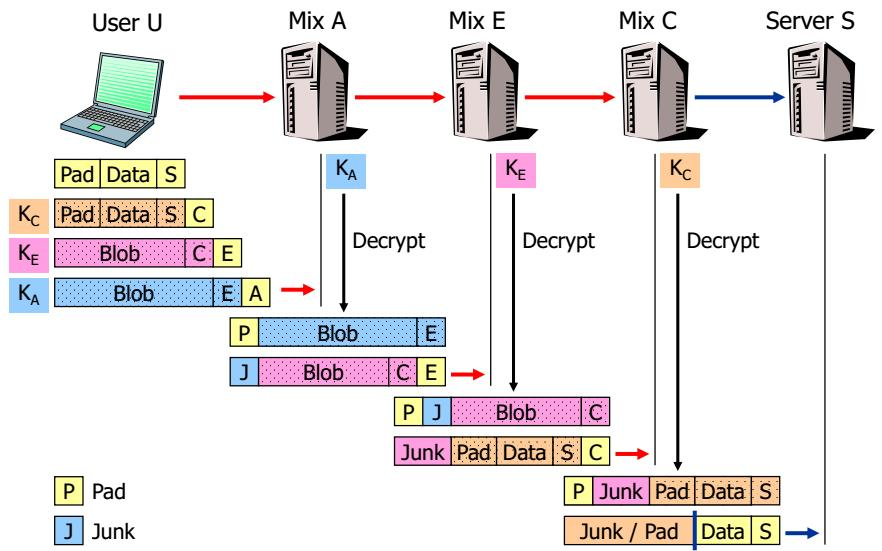
\includegraphics[width=0.7\linewidth]{images/onion_routing}
	\caption{Onion Routing}
	\label{fig:onionrouting}
\end{figure}

\subsubsection{Circuits}
Circuits werden Schritt für Schritt aufgebaut, wobei Perfect Forward Secrecy garantiert wird. Ebenfalls benutzt der Client keinen Public Key, weshalb er anonym bleibt. Die Circuit ID wird immer vom Absender gesetzt.
\begin{figure}[h]
\centering
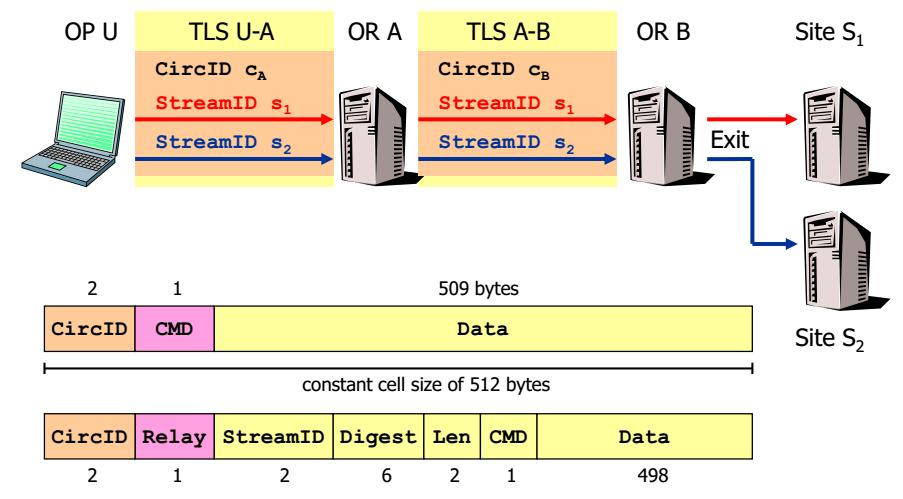
\includegraphics[width=0.7\linewidth]{images/tor_cells_circuits_streams}
\caption{Cells, Circuits und Streams}
\label{fig:torcellscircuitsstreams}
\end{figure}

\subsubsection{Vorgehen}
\begin{enumerate}
	\item Der Client sendet die erste Hälfte des DH Handshake verschlüsselt an den Entry Point. $g^X$ (Create Cell)
	\item Der Entry Point sendet die zweite Hälfte des DH Handshake, sowie einen Hash über den ausgehandelten Key ($K=g^{XY}$) zurück an den Client. $g^Y$(Created Cell)
	\item Nun muss der Circuit um weitere Nodes erweitert werden. Dazu sendet der Client ein Relay Extend Cell zum Entry Point, mit der Information, welcher der nächste Node im Circuit sein soll. Die Meldung enthält zusätzlich einen neuen ersten Teil des DH Handshake mit dem nächsten Node
	\item Der Entry Point leitet kopiert den ersten Teil des DH in eine Create Cell und leitet sie an den nächsten Node weiter. Ebenfalls wählt der Entry Point eine neue Circuit ID zwischen ihm und dem neuen Node.
	\item Der neue Node antwortet wieder mit einer Created Cell und der Entry Point mit einem Relay Extended. Nun kennt der neue Node und der Client den neuen ausgehandelten  Key $K_2 = g^{X_2 Y_2}$
	\item Dieser Schritt wird nun noch mindestens einmal wiederholt.
\end{enumerate}

\begin{figure}[h]
\centering
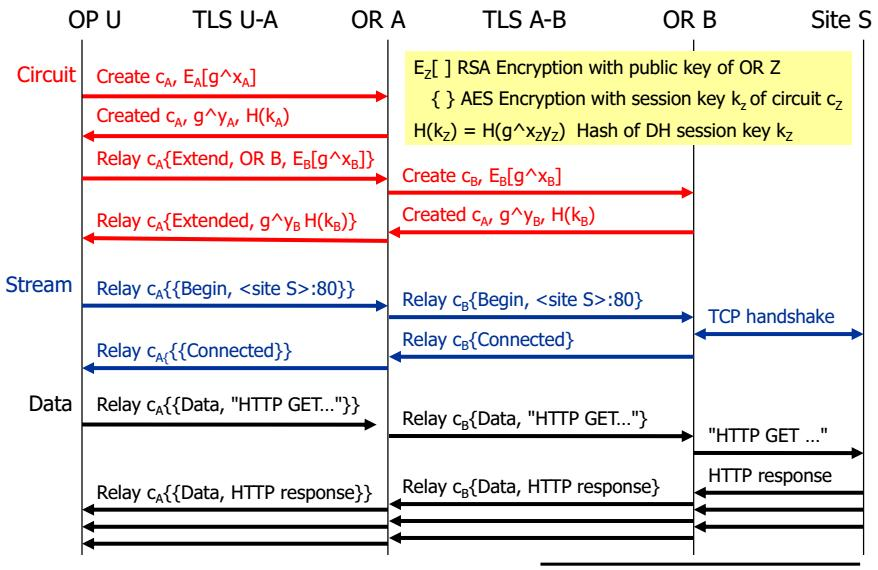
\includegraphics[width=0.7\linewidth]{images/tor_circuit_construction}
\caption{Erstellung eines Tor Circuit}
\label{fig:torcircuitconstruction}
\end{figure}


\subsection{Hidden Services}
\begin{enumerate}
	\item Ein beliebiger Nutzer möchte sensitive Daten über Tor verbreiten. Er setzt dafür einen Webserver auf und konfiguriert Tor so, dass die Daten auf dem Webserver gefunden werden könnnen (\lstinline|etc/tor/torrc| $\rightarrow$ \lstinline|HiddenServiceDir|).
	\item Nach dem Neustart wird ein Schlüsselpaar erstellt, das den Hidden Service identifiziert
	\item Der Hidden Service baut Tor Circuits zu zufälligen Introduction Points auf und sendet ihnen seinen Public Key. Danach erstellt er einen Hidden Service Descriptor. Dieser besteht aus genau diesen Introduction Points und seinem Public Key. Der Descriptor wird mit dem Private Key signiert und auf einen Verzeichnis Server geladen. Der Hidden Service ist nun verfügbar.
	\item Möchte der Client auf den Hidden Service zugreifen, muss er einen Hash über den Public Key des Service bilden. (\lstinline|16_char_hash.onion|). Mit diesem Hash kann der Service im Verzeichnisdienst abgefragt werden. Er erhält darauf die Liste der Introduction Points, sowie den Public Key. Der Client erhält den Public Key auf eine beliebige Art und Weise (weitersagen, über Tor, etc.)
	\item Der Client baut eine Verbindung zu einem zufälligen Rendezvous Point auf und übermittelt diesem ein One Time Secret. (Cookie) Dieses Cookie wird dort hinterlegt.
	\item Zusätzlich wird eine Verbindung zu einem der vorliegenden Introduction Points hergestellt. Der Client sendet dann eine mit dem Public Key verschlüsselte Introduction Meldung an einen ausgewählten Introduction Point und verlangt, dass die Meldung an den Hidden Service weitergeleitet wird. Diese Meldung enthält das One Time Secret (Cookie), der erste DH Teil, sowie der ausgewählte Rendezvous Point. 
	\item Der Hidden Service entschlüsselt die Meldung und weiss nun über den Rendezvous Point bescheid. Durch das enthaltene One Time Secret (Cookie) kann die Verbindung vom Rendezvous Point zwischen Client und Service verbunden werden. Dazu sendet der Hidden Service das Rendezvouz Cookie und der zweite DH Teil an den Rendezvouz Point.
	\item Beide können nun Daten austauschen ohne ihre gegenseitige Identität zu kennen. Ebenfalls weiss der Rendezvouz Point weder über Alice und Bob, noch die Daten die die beiden senden, bescheid!
\end{enumerate}

\begin{figure}[h]
\centering
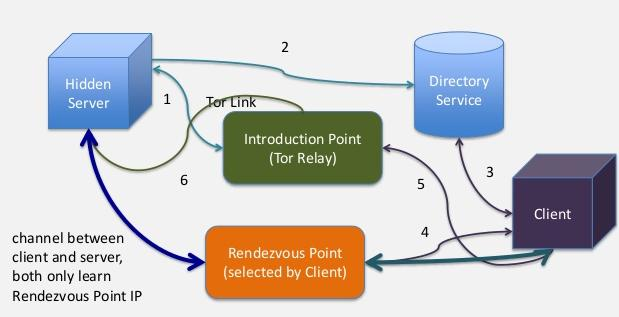
\includegraphics[width=0.7\linewidth]{images/hiddenservice}
\caption{Hidden Service}
\label{fig:hiddenservice}
\end{figure}

\subsubsection{RP: Rendezvous Point}
Der Rendezvous verbindet den Client mit dem Hidden Service. Wird er mit einer DDoS Attacke in die Knie gewungen, kommt keine Kommunikation zu stande.


\section{Firewalls}
Heutzutage sind alle Firewalls Stateful Inspection Firewalls. Früher waren die Firewalls nur Paketfilter, was zur Folge hat, dass man extrem viele Regeln hatte.
\begin{description}
	\item[Outer Perimeter] DMZ
	\item[Inner Perimeter] Intranet
	\item[Mission Cirtical Systems] HR, Finance, Know How
\end{description}

\begin{figure}[h]
\centering
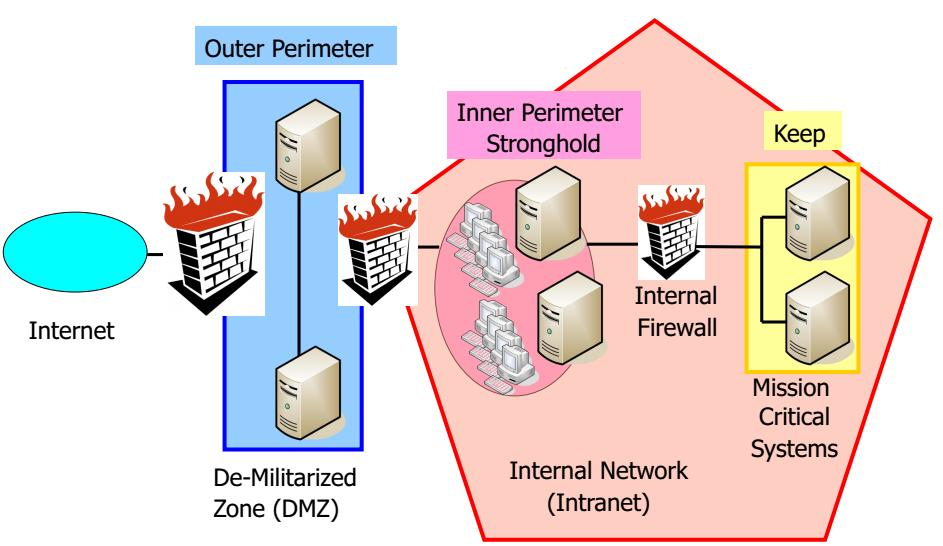
\includegraphics[width=0.7\linewidth]{images/firewall}
\caption{Firewalls}
\label{fig:firewall}
\end{figure}

\section{Intrusion Detection}
Firewalls können nicht sämtliche Angriffe zuverlässig abwehren. Aus diesem Grund sind Intrusion Detection Systeme nötig, um festzustellen ob, jemand die Firewalls überwinden konnte. Man unterscheidet zwischen zwei Typen von IDS.
\begin{description}
	\item[HIDS: Host-based IDS] Überwachen einzelne Hosts. Man installiert ein Stück Software auf dem Host, das als Sensor agiert und z.B die Logs durchforstet.
	\begin{itemize}
		\item Vorteile: Relative wenige False Positives
		\item Nachteile: Sieht nur einen Hosts und kann mit einem Rootkit unterwandert werden. Verursacht zusätzliche Last auf dem Host
	\end{itemize}
	\item[NIDS: Network IDS] Überwachen ganze Netwerk Segmente. Man verbindet spezielle NIDS Geräte mit dem Monitorport eines Switches/Router.
	\begin{itemize}
		\item Vorteile: Sieht ein grösseres Spektrum wie HIDS
		\item Nachteile: Hat Probleme mit verschlüsseltem Verkehr, benötigt zusätzliche Hardware
	\end{itemize}
\end{description}

\begin{figure}[h]
\centering
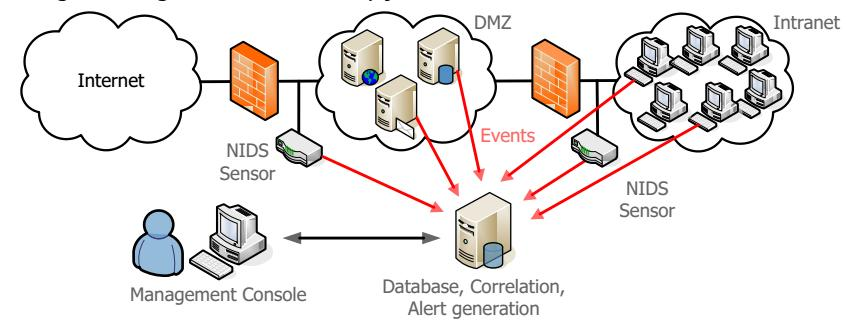
\includegraphics[width=0.7\linewidth]{images/hybrid_ids}
\caption{Hybrid IDS: HIDS kombiniert mit NIDS}
\label{fig:nids}
\end{figure}


\subsection{Terminologie}
\begin{description}
	\item[Sensor] Sensort der System und Netzwerkaktiviäten überwacht
	\item[Event] Ein Sensor generiert einen Event, wenn er es für Nötig hält, etwas zu melden.
	\item[Alert] Ein oder mehrere Events können in einem Alarm eskalieren (Abhängig von den konfigurierten Regeln). Ein Alert hat menschliche Interaktion zur Folge
	\item[Datenbank und Correlation Engine] Ein zentralisierter Host sammelt Events von verschiedenen Sensoren, korreliert diese und erstellt Alert wenn nötig
	\item[Management Console] Hierüber wird das IDS konfiguriert und Reports generiert
	\item[False Positive] Fehlerhafter ALert den von einem IDS ausgelöst wird
	\item[False Negative] Ein Angriff der von einem IDS nicht erkennt wird
\end{description}

\subsection{Erkennung}
IDS arbeiten mit zwei Techniken, um Angriffe zu erkennen. Aktuell domierniert die Signatur Variante, wobei auch Hybrid Variaten genutzt werden.

\paragraph{Signaturen}
Man erstellt Signaturen und prüft die Daten gegen diese Signaturen. z.B Suche nach \lstinline|/etc/passwd| in Paket. Das Problem bei dieser Variante ist, dass sie neuartigen Attacken oder Variationen (anderes Encoding, Fragmentierung, etc.) immer hinterherhinkt.

\paragraph{Anomaly Detection}
Man vergleicht die überwachten Daten mit jeden, die man als normal betrachtet.

\subsection{Reaktion}
Auf einen Alert kann ebenfalls auf verschiedenne Weisen reagiert werden
\begin{description}
	\item[Nichts Unternehmen] Nichts unternehmen und einfach nur Loggen
	\item[Manuell] Manuell intervenieren, was sehr langsam ist
	\item[Automatisch] Die Verbindung automatisch unterbrechen und dynamisch die Firewalls Rules anpassen
\end{description}

\subsection{Evasion}
\paragraph{Fragmentierung} IDS Systeme können auch umgangen werden, wenn man z.B die Pakete fragmentiert. (z.B \lstinline|nmap -f --send-eth|) Die meisten IDS Systeme sind aber standardmässig so eingestellt, dass sie die fragmentierten Pakete reassemblieren. Ebenfalls könnte die Reihenfolge der IP Fragmente geändert werden.

\paragraph{Verzögerung} Ein Port Scan könnte vom Angreifer verzögert werden, damit das IDS die einzelnen Zugriffsversuche nicht als einen zusammenhängenden Portscan erkennt.

\paragraph{Signatur ''anpassen''} Eine andere Variante wäre es, die Pakete so anzupassen, dass die Snort Rules (Signaturen) nicht mehr greifen. Dafür ist aber ein erweitertes Wissen über die Rules nötig.

\paragraph{SYN Scan} Ein Angreifer könnte bei einem Portscan,  nicht einen kompletten TCP Handshake durchführen (ACK dropen) und hoffen, dass der ISP nur komplette TCP Handshakes beachtet.

\paragraph{Distributed} Der Portscan von mehreren Clients aus durchgeführt werden.

\clearpage

\subsection{Snort}
Snort ist ein freies Network Intrusion Detection System (NIDS) und ein Network Intrusion Prevention System (NIPS). Es kann zum Protokollieren von IP-Paketen genauso wie zur Analyse von Datenverkehr in IP-Netzwerken in Echtzeit eingesetzt werden. 

\begin{lstlisting}
[alert|log|pass|activate|dynamic] [tcp|udp|icmp|ip] [src ip|any] [src port|any] [->|<>] [dest ip|any] [dest port|any] ( [option]:""; msg:""; )

// example
alert icmp any any -> 192.168.0.150 any (itype:8; msg:"ICMP Echo Request detected"; sid: 1000001)

// preprocessor (detects nmap -sS 192.168.0.0/24)
preprocessor sfportscan: proto { TCP } scan_type { all } sense_level { medium } watch_ip { 192.168.0.0/24 } logfile { /var/log/snort/portscan }

// reassembly fragmented packages
preprocessor frag3_global: max_frags 65536 
preprocessor frag3_engine: policy first detect_anomalies
\end{lstlisting}


\section{Network Access Controll}

Die Network Access Controll (NAC) ist eine Technologie, um unauthorisierte Zugriffe auf das Firmennetzwerk zu unterbinden. Mit NAC werden Clients während der Authentisierung auf Richtlinienkonformität geprüft. Neben einer Authentisierung wie bei MACSec (Kapitel \ref{sec:macsec-media-access-layer-security-ieee-8021ae}) ist es mit der NAC Policy Enforcement möglich, Client-Konfigurationen vorauszusetzen, wie z.B. bestimmte Betriebssystem- und Softwareversionen, Binary Integrity Checks oder Netzwerkkonfigurationen. Diese werden jeweils vom NAC Policy Enformcement Point vom Client abgefragt; je nach dem wird darauf ein bestimmter Zugang zum Netzwerk ermöglicht. \\\\
Virenverseuchten Computern kann so (im Prinzip) der Zugriff auf das Firmennetzwerk verboten werden; bei zu alten Software-Versionen könnte der Client in ein isolierte Umgebung (VLAN) eingebunden werden, um Updates durchzuführen. 

\subsection{Aufgaben}
Kernaufgabe sind:
\begin{itemize}
	\item eindeutige Identifizierung und Rollenverteilung von Nutzern und Geräten
	\item Wahrung von erstellten Sicherheitsrichtlinien
	\item Quarantäne und automatische Wiederherstellung nichtkonformer Endgeräte
	\item Verwaltung und Erstellung individueller Richtlinien und Rollen für verschiedene Nutzergruppen
\end{itemize}


\begin{figure}[h!]
\centering
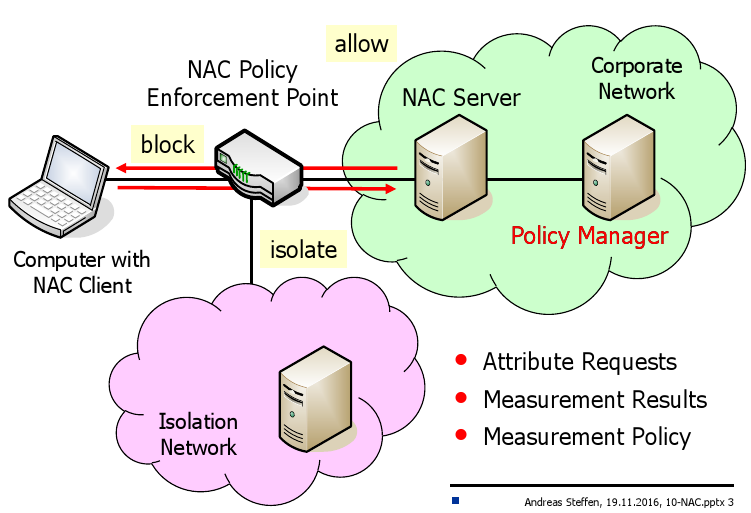
\includegraphics[width=0.7\linewidth]{images/network_access_control}
\caption{Network Access Control}
\label{fig:networkaccesscontrol}
\end{figure}

\clearpage

\subsection{TNC: Trusted Network Connect}
Im Gegensatz zu Network Access Control (NAC) und Network Access Protection (NAP), handelt es sich beim TNC-Konzept um eine offene Architektur für die Netzwerkzugangskontrolle. 
\subsubsection{Standard}
Es gibt bei der Trusted Computing Group und IETF einige Standards, welche allerdings noch in den Startlöchern sind, und einige proprietäre Lösungen (z.B. von Microsoft, Cisco und HP). Jeder Herrsteller ist befugt eigenen Attribute in seinem Namespace hinzuzufügen. Die Standardattribute des IETF können somit erweitert werden.


\begin{figure}[h!]
	\centering
	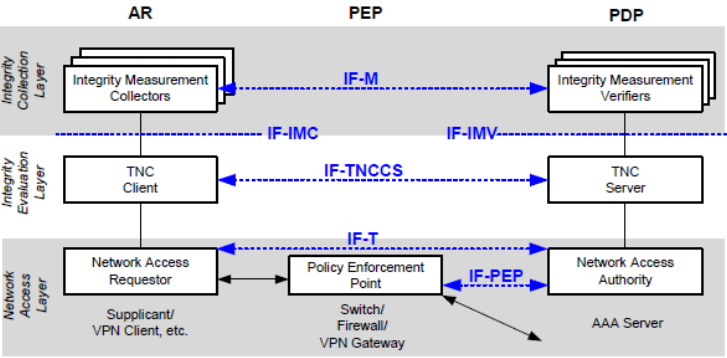
\includegraphics[width=0.7\linewidth]{images/nac_trusted_network_connect}
	\caption{Trusted Network Connect}
	\label{fig:nactrustednetworkconnect}
\end{figure}

Die Integrity Measure Collectors sammeln auf der Clientseite alle relevanten Informationen (Antivirus-Status, Netzwerk-Status, OS-Status etc.)

Über das IF-TNCCS (Interface-TNC Client Server Protokoll) wird der aktuelle Stand des Clients an den Server gesendet. Der TNC-Server entscheidet daraufhin, ob und was für ein Zugriff erlaubt wird.

\subsubsection{Verbindungsaufbau}

Funktioniert über IKEv2 with EAP. Um MITM zu verhindern, kann der Client zuerst ein Zertifikat beim Authentisierungsserver anfragen (siehe Kapitel zu IPSec \ref{sec:ipsec-internet-protocol-security}), daraufhin finden eine EAP-Identity \& Challange-Responste mit PSK statt.

Üblicherweise findet die Kommunikation über ein TNC IF-T Protokoll via IKEv2 EAP-TTLS. Dies ist allerdings nicht der Standard (dank Intervention von Cisco).

Standardmässig findet die Kommunikation über ein spezielles Tunneled-EAP-Protokoll statt.

\subsubsection{Forcierung der Polycies}

Üblicherweise wird die Policy einmal beim einwählen in das Netzwerk sowie periodisch geprüft (z.B. alle 20 Sekunden). 

\subsubsection{Problem des ''Lying Clients''}
Die Authentizität der Antwort des Clients kann mit dem TPM (siehe Kapitel \ref{sec:tpm}) verifiziert werden.

\subsubsection{Terminologie}
\begin{description}
	\item[TNC: Trusted Network Connect] Offene Architektur zur Netzwerkzugangskontrolle von TCG
	\item[AR: Access Requestor] Ersucht Zulassung in ein Netzwerk
	\item[PEP: Policy Enforcement Point] Setzt die Richtlinien des PDP bezüglich Netzwerkzugang durch. (z.B verschieben in eine isolierte Zone)
	\item[PDP: Policy Decision Point] Trifft die Authorisierungsentscheidungen, bei einer Anfrage durch den AR.
	\item[TNCC: TNC Client] Der Client kommuniziert über das IF-TNCCS Interface mit dem Server.
	\item[TNCS: TNC Server] Der Server kommuniziert über das IF-TNCCS Interface mit dem Client.
	\item[IMC: Integrity Measurement Collectors] Erlaubt TNCC und TNCS Plugin Komponenten von anderen Hersteller zu verwenden. Die gesammelten Daten werden über das IF-IMC Interface an den TNC Client gesendet. 
	\item[IMV: Integrity Measurement Verifier] Erlaubt TNCC und TNCS Plugin Komponenten von anderen Hersteller zu verwenden. Die Daten werden über das IF-IMV Interface an den TNC Server übertragen.
	\item[PTS: Platform Trust Service]
	\item[MAP: Metadata Access Point] Speichert und liefert Statusinformationen zu einem AR, die z.B im PDP/PEP benötigt werden.
\end{description}
\begin{figure}[h]
\centering
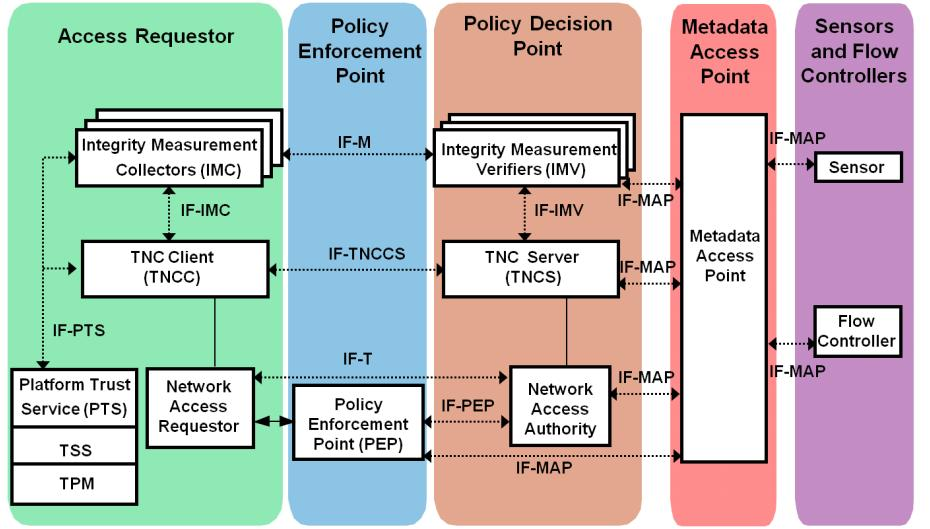
\includegraphics[width=\linewidth]{images/tnc_framework}
\caption{TNC Framework er Trusted Computing Group}
\label{fig:tncframework}
\end{figure}

\section{Buffer Overflow}
Normalerweise werden Buffer Overflow Attacken Remote ausgeführt. Damit die Attacke nicht zu viel Schaden ausrichten kann, sollten Server Daemon's nie mit root Rechten ausgeführt werden. Heutzutage sind Buffer Overflows nicht mehr ganz trivial durchzuführen. Die meisten aktuellen Angriffe gehen öfters auf den Heap. \\


Das Ziel des Buffer Overflows ist es, die Rücksprungadresse (Instruktionspointer) auf dem Stack zu manipulieren, dass dieser auf den Exploit zeigt. Damit die Exploits robuster werden, wird am Anfang NOP (No Operation) hinzugefügt und die neue Rücksprungadresse (EIP) mehrere Male am Schluss angehängt wird. Somit hat man mehr spielraum, um die Rücksprungadresse korrekt zu überschreiben.

\begin{itemize}
	\item Nie \lstinline|strcpy()| verwenden sondern \lstinline|strncpy()|
	\item \lstinline|execve()| übernimmt den aktuellen Prozess.
\end{itemize}

\begin{figure}[h]
\centering
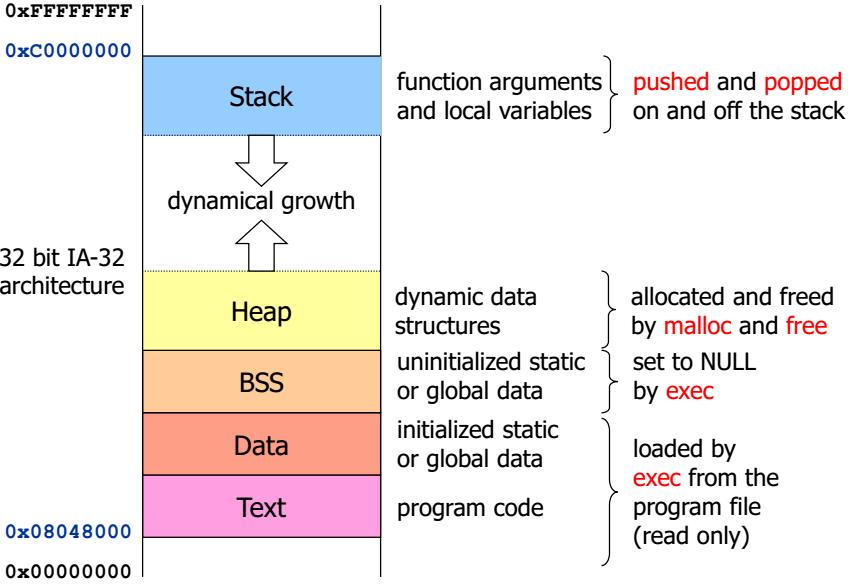
\includegraphics[width=0.7\linewidth]{images/memory_organization}
\caption{Virtual Process Memory Organization}
\label{fig:memoryorganization}
\end{figure}

\begin{description}
	\item[IP: Instruction Pointer] Adresse des nächsten Befehls (\%eip Register)
	\item[SP: Stack Pointer] Zeigt immer auf TOS (\%esp Register). Je tiefer die Adresse desto grösser ist der Stack.
	\item[BP: Base or Frame Pointer] Speichert den letzten Stackpointer (\%ebp Register)
	\item[call] call wirft die nächste Adresse auf den Stack,  damit nach Ablauf des Stackframes am richtigen Ort weitergefahren wird.
\end{description}

\subsection{Schutz}
\begin{description}
	\item[ASLR: Address Space Layout Randomization] Der Anfang des Stacks wird zufällig gewählt. Dies kann jedoch umgangen werden, wenn man die Adresse einer bekannten Umgebungsvariable kennt und dann das Offset ausrechnet.
	\item[Canaries] Werden zwischen Buffer und EIP zwischengeschoben. Die Canaries beginnen mit 0x00 und sind ansonsten komplett zufällig. Wird ein Buffer überschrieben, wird auch das Canarie überschrieben. Danach wird das Canarie aktuelle Canarie mit dem gemerkten XOR verknüpft und so ein allfälliger Buffer Overflow detektiert.
	\item[Exetuable Space Protection (Non-eXexute, NX bit)] Markiert das physische Memory als nicht ausführbar (Stack, Heap). Funktioniert nur auf 64Bit Systemen und in 32Bit Systememn mit aktiviertem PAE Adressierungsmodus.
\end{description}

\section{Smartcards}
Da Schlüssel auf der Festplatte rsp. Memory eines Notebooks nicht sicher sind, sollten Verschlüsselungs und Signatur-Keys immer auf einer Smartcard gespeichert werden. Von diesen ist es extrem schwierig, den Key zu klauen. Ein möglicher Nachteil ist es, dass dem Chipkarten-Hersteller vertraut werden muss, dass er einen zuverlässigen Schlüssel mit viel Entropie auf der Karte generiert.

\begin{itemize}
	\item Chipkarten haben oft eine tiefe Taktfrequenz, damit weniger Leistung benötigt wird.
	\item Chipkarten haben eine erhöhte physiche Sicherheit gegenüber herkömmlichen Prozessoren.
	\item Wegen der mechanischen Belastung, sind Chipkarten Prozessor sehr klein (2-3mm)
	\item Die kontaktlosen Zahlungskarten operieren auf der 13.56MHz Frequenz. Man muss deshalb so nah an den Leser gehen, damit genügend Spannung für den Kartenprozessor übertragen werden kann. (für die Spannungsübertragung ist eine magnetische Kopplung nötig)
\end{itemize}

\subsection{NFC: Near Field Communication}
Bei NFC gibt es das Problem, dass die Übertragung nicht sicher ist, wenn das Smartphone verseucht ist. Die einzige Lösung wäre es, dass die Mobile App über die sichere SIM Karte mit dem NFC Controller kommuniziert. Da die SIM Karte aber Eigentum der Netzbetreiber ist, wollen diese eine grosse Provision, weshalb die Kommunikation nach wie vor direkt auf den NFC Controller geht. Der NFC Controller kommuniziert mit dem Lesegerät. Es können dann beliebig viele Abbuchungen getätigt werden.

\subsection{Memory Layout}
\begin{description}
	\item[ROM] Betriebssystem
	\item[EEPROM] Keys
	\item[RAM] Zwischenspeicher für Berechnungen
\end{description}
\begin{figure}[h]
\centering
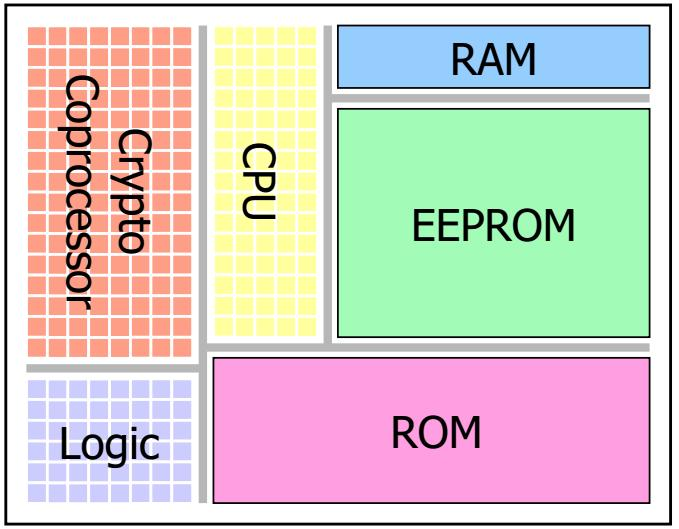
\includegraphics[width=0.5\linewidth]{images/card_memory_layout}
\caption{Memory Layout}
\label{fig:cardmemorylayout}
\end{figure}

\subsection{PKCS \#15: Cryptographic Token Information Format}
Es gibt ein Master File (Root Directory) und mehrere Dedicated (Folder) und Elementry Files (Daten). Ein Filename besteht aus 2Bytes (meist HEX). Die Anzahl Schreibzugriffe ist begrenzt. 

\begin{figure}[h]
\centering
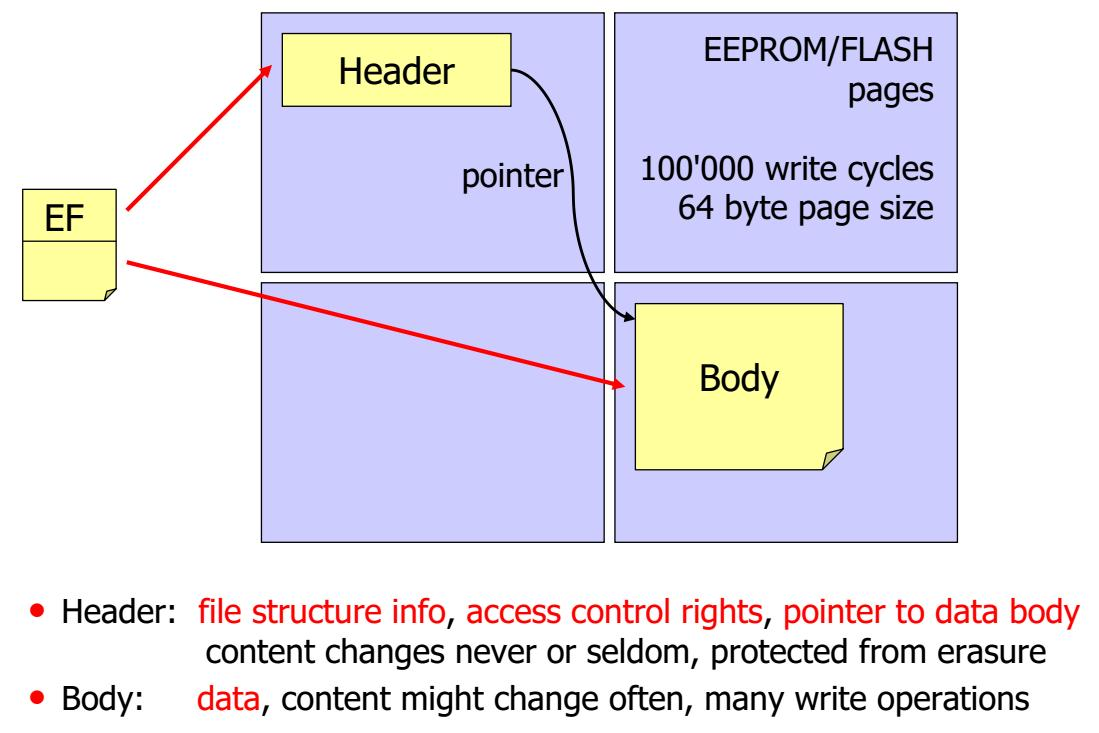
\includegraphics[width=0.5\linewidth]{images/smart_card_file_structure}
\caption{Smart Card File Struktur}
\label{fig:smartcardfilestructure}
\end{figure}

\begin{figure}[h!]
	\centering
	\includegraphics[width=0.7\linewidth]{images/pkcs15}
	\caption{PKCS 15 Filesystem}
	\label{fig:pkcs15}
\end{figure}

\begin{description}
	\item[MF] Das Root File existiert immer (FID=3F00)
	\item[DF: Directory File] Ein Ordner
	\item[EF: Elementary File] Ein Daten File
	\item[Cert] Beinhaltet das Zertifikat
	\item[PIN und PUK \#1] Reservierte FID=0000
	\item[PIN und PUK \#2] Reservierte FID=0100
	\item[FID=2F00] Dieses standardisierte Verzeichnis hält einen Zeiger auf das PKCS\#15 Applikationsverzeichnis mit der FID=5015
	\item[PKCS15] PKCS\#15 Applikationsverzeichis mit der FID=5015, enthält die eigentlichen Daten (Zertifikate und Schlüssel). Die Daten wiederum können sich sowohl im Verzeichnis 5015, als auch in jedem beliebigen anderen Verzeichnis auf der Chipkarte befinden.
	\item[ODF] Objektverzeichnis ist die wichtigste Datei. Es enthält einen Zeiger auf das aktuell verwendete Verzeichnis, welches wiederum einen Pointer auf das eigentliche Objekt hält.
\end{description}


\subsection{Auslesen}
Angriffe auf Smartcards sind sehr aufwändig und schwierig.
\begin{itemize}
	\item Möchte man den Chip auslesen muss die Passivationsschicht chemisch entfernt werden. Die Chiphersteller haben aber Funktionalitäten implementiert, damit dies bemerkt wird. 
	\item Hat man physischen Zugriff auf eine Smartcard, kann man diese mit Kältespray besprayen und in flüssiges Helium werfen. Somit wird der RAM Zustand über mehrere Wochen haltbar machen, weshalb man das RAM zu einem späteren Zeitpunkt mit einem Elektroden Mikroskop analysieren kann.
	\item Mittels Leistungs- und Zeitanalyse kann auf die Operation geschlossen werden. Deshalb versuchen die Hersteller einen möglichst konstanten Leistungsverbrauch zu erreichen.
\end{itemize}

\subsection{PKCS\#11: Cryptographic Token Interface Standard}
PKCS\#11 ist ein C API, welches die Smartcard als Objekt modelliert. 

\subsection{EMV: Europay, Mastercard, Visa}
EMV ist ein Standard für interoperable Kredit- und Debitkarten. Der Standard ist öffentlich verfügbar und setzt auf einen kopiergeschützen Chip anstatt auf einen Magnetstreifen. Es können RSA-, oder Elliptic Curve-Keys für die Authentifizierung der Karte verwendet werden. Die verbreitung ist mit Ausnahme der USA (2\%) und Asien (40\%) recht gut.


\section{PTS: Platform Trust Service}
\subsection{TPM: Trusted Platform Module}\label{sec:tpm} 
Das TPM ist ein Mikrochip mit dem Manipulationen an Software erkannt werden können. Zu diesem Zweck sammelt und speichert das TPM Daten, über vertrauenswürdige, extern ausgeführte Software. Stellt das TPM Veränderungen von Merkmalen an der Software fest, verweigert es den Zugriff auf den Schlüssel, mit der die Daten ver- und entschlüsselt werden. TPM Module waren früher eigene Chips auf dem Motherboard, sie werden jedoch immer mehr in die CPU integriert. \\\\
Ist ein TPM Chip auf dem PC Motherboard vorhanden, nimmt das OS während des gesamten Boot-Prozesses Messungen an den Treibern, ausgeführten Programmen, Libraries und geladenen Dateien vor und hasht die Messwerte in die \gls{pcr} des TPMs. Die gehashten Messwerte werden für die Attestation bei einem Firmennetzwerk gebraucht. Das Netzwerk setzt Policies vorraus, die ein Client erfüllen muss. Die PCR Werte werden z.B über das TNC Protokoll übertragen. 

\begin{description}
	\item[Endorsement Key] Der Endorsment Key ist fixes 2048 Bit langes RSA Schlüsselpaar, dass einem TPM zugeordnet und kann nicht verändert werden kann. Das Schlüsselpaar wird innerhalb des Chips verwaltet, wobei der private Teil von aussen nicht zugreifbar ist. 
	\item[SRK: Storage Root Key] Vom SRK werden alle weiteren Keys abgeleitet. Der 2048 Bit lange RSA Key basiert auf dem Endorsement Key und einem Nutzer spezifischen Passwort. 
	\begin{itemize}
		\item AIK: \textbf{Attestation Identiy Keys}: Der Attestation Key wird verwendet, da der Endorsement Key einzigartig ist und somit Rückschlüsse auf den Benutzer gezogen werden könnten. Attestation Keys sind nicht migrierbar und dürfen vom TPM nur für die \textbf{Digitale Signatur} von Werten eingesetzt werden, welche im Platform Configuration Register (PCR) abgelegt werden (Attestation). PCR sind ein Teil des flüchtigen Speichers im TPM und für die Speicherung von Zustandsabbildern der aktuellen Konfiguration von Soft- und Hardware zuständig.
		\item AIK Zertifikat: Wird für die verfikation einer AIK Signatur benötigt. Das Zertifikat wird von einer vertrauenswürdigen Privacy CA signiert und enthält einen Public Key. Mit dem Public Key kann die Signatur überprüft werden. Das Zertifikat wird nur ausgestellt, wenn die CA eine eindeutige Zuordnung zwischen AIK und TPM-EK vorgenommen werden kann. Dazu wird 
		\item SigK: Signing Keys
		\item BindK: Binding Keys
		\item MigrK: Migration Keys
		\item SymK: Symmetric Keys
	\end{itemize}
\end{description}

\begin{figure}[h!]
	\centering
	\includegraphics[width=0.9\linewidth]{images/measure_boot}
	\caption{Measure Boot}
	\label{fig:measureboot}
\end{figure}


\begin{figure}[h]
	\centering
	\includegraphics[width=0.5\linewidth]{images/tpm_architecture}
	\caption{TPM Architecture}
	\label{fig:tpmarchitecture}
\end{figure}

\subsection{Binding}
Das TPM kann Schlüssel auch ausserhalb des Trust Storage (z. B. auf der Festplatte) speichern. Diese werden ebenfalls in einem Schlüssel-Baum organisiert und deren Wurzel mit einem Key im TPM verschlüsselt. Somit ist die Anzahl der sicher gespeicherten Schlüssel nahezu unbegrenzt.

\subsection{Sealing}
Durch Bilden eines Hash-Wertes aus der System-Konfiguration (Hard- und Software) können Daten an ein einziges TPM gebunden werden. Hierbei werden die Daten mit diesem Hash-Wert verschlüsselt. Eine Entschlüsselung gelingt nur, wenn der gleiche Hash-Wert wieder ermittelt wird (was nur auf demselben System gelingen kann). Bei Defekt des TPM muss nach Aussagen von Intel die Anwendung, die Sealing-Funktionen nutzt, dafür sorgen, dass die Daten nicht verloren sind.


\subsection{SRTM: Static Root of Trust for Measurement}
Bei SRTM wird von unten her die geladenen DLL's gehashed und iterativ überschrieben. Dazu muss man in erster Linie dem TPM vertrauen. Dieses wird gehashed und so geht es über das CRTM, BIOS, Boot Loader, OS, Application, usw. weiter.

\subsection{DRTM: Dynamic Root of Trust for Measurement}
Der Ladeprozess eines Binaries wird erst ausgeführt, wenn die Signatur davon Stimmt. (Umsetzung z.Z. via Intel vPro / Trusted Execution Technology für VMs. Dadurch entsteht aber eine Abhängigkeit zur Hardware.)

\subsection{Anwendungsbereiche}
\begin{itemize}
	\item Verschlüsselung von Daten mit symmetrischen Keys
	\item Authentifizierung bei Remote Systemem durch hinterlegte Zertifikate 
	\item Überprüfung der Systemintegrität (Pre-Boot). Das Resultat von SRTM wird im TPM gespeichert und kann von autorisierten Dritten online abgefragt werden. 
	\item Plattformbescheinigung (Remote Attestation)
\end{itemize}

\subsection{PTT: Platform Trust Technology und TrustZone}
PTT ist wie TPM aber in Software von Intel. Das gleiche gibt es auch von ARM und heisst dort TrustZone.

\section{Secure Boot}
Secure Boot ist ein Teil der UEFI-Spezifikation, der die Echtheit bzw. Unverfälschtheit von wichtigen Software-Teilen der Firmware garantieren soll. Kritische Teile der Firmware, wie der OS-Loader, sollen nur mehr dann ausgeführt werden, wenn sie zuvor durch eine vertrauenswürdige Institution dazu autorisiert wurden. Dadurch werden unter anderem Rootkits ausgeschlossen, die sich schon vor dem Boot des Betriebssystems (OS) einnisten.
\\ \\
Durch Signaturen von einem Zertifikat, dessen Public Key im UEFI hinterlegt ist, wird verhindert, dass nicht vertrauenswürdige Software-Teile ausgeführt werden.
\\ \\
Die Schlüssel in der UEFI-Firmware prüfen die Authentizität von z.B. Bootloadern. Ein Bootloader wird nur dann ausgeführt, wenn er eine gültige Signatur hat. Kann eine Signatur nicht überprüft werden bzw. ist sie nicht gültig wird das System am Starten gehindert. Entspricht z.B. die Signatur des Bootloaders nicht der, die die UEFI-Firmware erwartet, startet das System nicht. 
\begin{description}
	\item[PK: Platform Key]  \hfill \\
	Sobald der Platform Key in UEFI geschrieben wird, wechselt das UEFI von Setup Mode in den User Mode. Normalerweise wird ein Notebook bereits mit einem Platform Key des Herstellers ausgeliefert. Der PK stellt eine Vertrauensbasis zwischen dem Platform Besitzer und der Firmware her.
	\item[KEK: Key Exchange Keys] \hfill \\
	Der KEK wird benötigt um Zertifikate in die Allowed/Forbidden Database speichern zu können. Der KEK muss mit dem private Platform Key signiert werden, damit der KEK verwendet werden kann. Der KEK stellt eine Vertrauens Basis zwischen dem OS und der Firmware her.
	\item[Platform Key Database] Objekte zur Modifizierung der KEK's
	\item[Key Exchange Key Database] Beinhaltet jene Trust-Objekte, welche die Allowed und Forbidden Signature Database modifizieren dürfen	
	\item[Allowed Database] \hfill \\
	Hier sind die Zertifikate von Software Signers hinterlegt (Microsoft).
	\item[Forbidden Database] \hfill \\
	Enthält die Revoked Signing Zertifikate. Damit können gewisse Software in die Blacklist geschrieben werden.
\end{description}

\subsection{Ablauf}
\begin{enumerate}
	\item Der OS Loader Code muss mit dem Private Key eines Software Signers signiert sein
	\item Das Zertifikat des Software Signers muss sich in der Allowed Database des UEFIs befinden. Das Zertifikat kann nur im UEFI gespeichert werden, wenn es mit einem KEK signiert ist, dessen KEK Zertifikat sich schon im UEFI befindet. 
	\item Ein KEK Zertifikat kann nur ins UEFI importiert werden, wenn es 
	mit dem PK des Hardwareherstellers signiert ist.
	\item Das PK Zertifikat des Hardwarehersteller muss bei der Aktivierung des Secure Boot Modus ins UEFI importiert werden
\end{enumerate}

\begin{figure}[h!]
	\centering
	\includegraphics[width=0.8\linewidth]{images/secureboot}
	\caption{Secure Boot}
	\label{fig:secureboot}
\end{figure}
\begin{figure}[h!]
	\centering
	\includegraphics[width=0.9\linewidth]{images/secure_boot}
	\caption{Secure Boot unter Windows 8}
	\label{fig:secureboot}
\end{figure}


\section{Virtualization}
\begin{figure}[h]
\centering
\includegraphics[width=0.5\linewidth]{images/virtualization_rings}
\caption{Virtualisierung: Protection Rings}
\label{fig:virtualizationrings}
\end{figure}

\subsection{Hypervisor Typen}
Man unterscheidet zwischen zwei Typen von Hypervisor:

\begin{itemize}
	\item Type1 (native): VMware ESX, Microsoft Hyper-V, Xen, Oracle VM Server (\textbf{Ring -1 (bare metal)})
	\item Type2 (hosted): KVM, VirtualBox, VMWare Workstation
\end{itemize}

\begin{figure}[h]
\centering
\includegraphics[width=0.5\linewidth]{images/hypervisor_types}
\caption{Hypervisor Types}
\label{fig:hypervisortypes}
\end{figure}

\subsection{Qubes OS}
Qubes OS ist ein OpenSource Betriebssystem welches versucht durch Isolation den gewöhnlichen Desktop sicherer zu machen. Qubes OS basiert auf Xen und nutzt AppVM's für die Separierung. Dazu setzt es auf Virtualisierung, um Programme und Systemkomponenten (z.B Netzwerkstack) voneinander zu isolieren. Damit soll die Komprommitierung einese Teils des System, die Integrität des restlichen Systems nicht beeinflussen. 

\subsubsection{GUI Protokoll}
Für die Kommunikation zwischen den Qubes Instanzen wird ein Shared Memory verwendet. Nachrichten werden über das Xen vchan Protokoll übertragen. Die eigentliche Grafikausgabe ist ebenfalls via Shared Memory implementiert. Die lokalen X Server der VMs verwenden einen speziellen Treiber der einfach in einen Framebuffer zeichnet, der nicht mit echter Hardware verknüpft ist. Dieser Memorybereich wird dann in dom0 in den dortigen X Server gemappt. Xen stellt dabei sicher, dass der Memory Bereich auch tatsächlich zur jeweiligen VM gehört. Dank diesem Vorgehen, hat nur dom0 auf den grafischen Output mehrere VM's Zugriff. Die jeweiligen VMs haben keinen direkten Zugang zur Grafikkarte oder die Framebuffer der anderen VMs. Damit werden Informationsleaks via Grafikausgabe verhindert. Dom0 hat als einzige direkten Zugriff auf die Tastatur. 

\section{Selbststudium}
\subsection{Tor}
Siehe \ref{sec:tor}

\subsection{Secure Boot}
Was sind die Eigenschaften von UEFI, TPM, Virtual Smart Card?
\begin{itemize}
	\item UEFI -> Secure Boot
	\item TPM -> Measure Boot 
	\item XP SP2: ASLR, Firewall on by Default (erste wichtige Security Updates)
	\item Vista: TPM für Bitlocker
	\item Windows 7: Grösster Schritt wegen SDL: Secure Development Lifecycle, Biometric Authentication
	\item Windows 8: UEFI Secure Boot -> Measure Boot und Remote Attestation (UEFI ist Pflicht, sonst kein Lizenzkleber)
	\item Das UEFI 2.3.1 ist ein eigenes OS mit TCP/IP Stack -> Man muss es deshalb unbedingt mit TPM überprüfen. (Gefahr von nach Hause telefonieren)
	\item \textbf{VCS: Virtual Smart Card}: Beliebig viele Smartcards. Das TPM verhält sich wie eine ständig eingesteckte Smartcard.
	\item Seit Windows 8 können Anti Malware Programme über eine Hook eingehängt werden. Dies erlaubt es , dass die Anti Malware frühere Dinge im Boot Prozess zu überprüfen.
	\item Man unterscheidet zwei Typen von Unternehmen
	\begin{itemize}
		\item Jene die merken, dass sie gehackt wurden
		\item Jene die nicht merken, dass sie gehackt wurden.
	\end{itemize}
\end{itemize}

\paragraph{Bekannte Threads}
\begin{itemize}
	\item Script Kitties
	\item Cybercrime
	\item Attacken auf die Fortune 500
	\item Hoffen, dass man nicht gehackt wird.
\end{itemize}

\paragraph{Neuartige Threads}
\begin{itemize}
	\item Cyber Spionage, Cyber Warfare, State Sponsored Actions
	\item Alle Organisationen werden angegriffen
	\item Man wird gehackt. Es geht darum, wie man damit umgeht.
\end{itemize}




\appendix

% Code Listings
\lstlistoflistings

% List of figures
\listoffigures

% List of tables
\listoftables

% Bibliography
\bibliographystyle{plain} 
\bibliography{literatur}

\end{document} 